% options:
% thesis=B bachelor's thesis
% thesis=M master's thesis
% czech thesis in Czech language
% slovak thesis in Slovak language
% english thesis in English language
% hidelinks remove colour boxes around hyperlinks

\documentclass[thesis=B,czech,hidelinks]{FITthesis}[2012/06/26] %documentclass ... typ dokumentu (definovany v souboru .cls)

\usepackage[utf8]{inputenc} % LaTeX source encoded as UTF-8

\usepackage{graphicx} %graphics files inclusion
\usepackage{adjustbox}
\usepackage{multirow,tabularx}
\usepackage{xargs} 
\usepackage[pdftex,dvipsnames]{xcolor} 
\usepackage[colorinlistoftodos,prependcaption,textsize=tiny]{todonotes} 
\usepackage{svg}

% \usepackage{amsmath} %advanced maths
% \usepackage{amssymb} %additional math symbols

\usepackage{dirtree} %directory tree visualisation

% % list of acronyms
%\usepackage[acronym,nonumberlist,toc,numberedsection=autolabel]{glossaries}
%\iflanguage{czech}{\renewcommand*{\acronymname}{Seznam pou{\v z}it{\' y}ch zkratek}}{}
%\makeglossaries

\newcommand{\tg}{\mathop{\mathrm{tg}}} %cesky tangens
\newcommand{\cotg}{\mathop{\mathrm{cotg}}} %cesky cotangens
\newcommandx{\note}[2][1=]{\todo[linecolor=OliveGreen,backgroundcolor=OliveGreen!25,bordercolor=OliveGreen,#1]{#2}}
\newcommand{\code}[1]{\texttt{#1}}
\newcommand\tab[1][1cm]{\hspace*{#1}}

\department{Katedra softwarového inženýrství}
\title{Interaktivn{\' i} ovl{\' a}d{\' a}n{\' i} PC hry pomoc{\' i} chytr{\' e}ho telefonu}
\authorGN{Marek} 
\authorFN{Foltýn} 
\authorWithDegrees{Marek Foltýn} 
\supervisor{Ing. Filip K{\v r}ikava, Ph.D.}
\acknowledgements{Chtěl bych poděkovat vedoucímu práce Ing. Filipu K{\v r}ikavovi, Ph.D., za pomoc a~p{\v r}íkladné vedení. Dále pak své manželce Veronice Foltýnové za trpělivost a~ochotu vytvá{\v r}et prost{\v r}edí vhodné k~tvorbě bakalářské práce, 
rodičům a~celé mé rodině za velkou podporu ve všech směrech. Děkuji také všem, kdo se podíleli na testování hratelnosti hry.}
\abstractCS{Tato bakalářská práce se zabývá tvorbou systému pro ovládání PC hry pomocí mobilního telefonu. Hlavním cílem je obohacení herního zážitku pomocí interaktivních prvků, které jsou na mobilních telefonech k~dispozici. Součástí práce je analýza způsobů ovládání her, přehled interaktivních technologií v~mobilních telefonech a~samotná tvorba komunikačního systému, který je demonstrován na jednoduché hře. }
\abstractEN{The main purpose of this thesis is to create an interactive PC game control system using smartphones in order to enhance the game experience. The thesis contains the analysis of different ways how a~PC game can be controlled, the overwiev of interactive mobile technologies and also the communication system implementation, which is demonstrated in a~simple game. }
\placeForDeclarationOfAuthenticity{V~Praze}
\declarationOfAuthenticityOption{1} %volba Prohlášení (číslo 1-6)
\keywordsCS{interaktivní ovládání, počítačové hry, smartphone, komunikační systém, Cocos2d-x, RakNet}
\keywordsEN{interactive control, computer games, smartphone, communication system, Cocos2d-x, RakNet}

\begin{document} 

% \newacronym{CVUT}{{\v C}VUT}{{\v C}esk{\' e} vysok{\' e} u{\v c}en{\' i} technick{\' e} v Praze}
% \newacronym{FIT}{FIT}{Fakulta informa{\v c}n{\' i}ch technologi{\' i}}
\begin{introduction}
Videohry existují od počátku prvních počítačů. \cite{rylich} Jejich možnosti jsou úzce spjaty s~vývojem výpočetního a~grafického výkonu, hardwaru a~dalších souvisejících technologií. Neustálé zmenšování součástek v~současné době nabízí vysoký výkon ve velmi malých strojích. \cite{kupi} Na moderní typy hardwaru se adaptovaly i~hry. Jsou vyvíjeny pro přenosná zařízení, jako například mobilní telefony nebo tablety. Lidé tak mohou hrát doslova kdekoli. Nemusí být doma, jako je tomu u~klasických počítačových a~konzolových her, ale mohou hrát v~čekárně, ve škole o~přestávce, na cestě a~podobně.

Mobilní zařízení jsou v~dnešní době velmi úzce propojená s~lidmi a~jejich životem. Na základě toho se nabízí otázka, zda~by tyto nové možnosti mohly nějakým způsobem obohatit herní interakci mezi lidmi. Existuje několik směrů, které se o~tento cíl snaží:

Způsobem, jak dosáhnout lepší mezilidské interakce ve hře, je hra více hráčů, tzv. \textit{multiplayer}. Jedná se o~typ, kdy na~sebe v~herním světě reaguje více hráčů, ať už v~reálném čase, nebo pomocí sdílení pokroku ve hře (např. žebříčky s~výsledným skóre). Obě tyto varianty sice poskytují informace o~hře ostatních lidí, avšak ve spojení s~internetem nemají zásadní vliv na mezilidskou komunikaci: spíše vylepšují vlastnosti herního světa, aby zlepšily hráčův zážitek. Jako příklad uvedu běžného hráče počítačové hry, který hraje doma v~pokoji multiplayerovou online hru přes internet: Sice se pohybuje ve stejném virtuálním světě jako další hráči, ale vliv na mezilidskou komunikaci je minimální. Dalším příkladem může být herní interakce pomocí sociálních sítí. Kromě svého pokroku ve hře vidí hráč i~pokrok ostatních lidí a~může ovlivnit jejich hru. Opět se ale nejedná o~sociální interakci ve smyslu fyzické přítomnosti. Virtuální realita zde tvoří pouze prostor, skrz který ostatní hráči sledují jeden druhého.

I~přes tyto nevýhody existují způsoby, jak spojit virtuální realitu ve hře s~širší mezilidskou komunikací. Jedním z~nich je hra v~lokální síti, kdy jsou hráči fyzicky přítomni na jednom místě (pokoj, garáž). Hráči prožívají stejný herní zážitek jako v~případě hry přes internet, avšak umocněný přítomností ostatních hráčů. Reakce během hry pak mohou obsahovat prvky komunikace typické pro mezilidský kontakt ve fyzické přítomnosti: zvuk, vizuální a~fyzický kontakt a~podobně.

Dalším způsobem je hra na jednom PC nebo konzoli. Pro tento způsob je typické sdílení jedné obrazovky (monitor, televize) a~případně ovládacích periferií (klávesnice). Herní svět pak netvoří virtuální \emph{bariéru}, přes kterou hráč vnímá ostatní lidi, ale stává se součástí prostředí společně s~lidmi, podobně jako například stolní hry.

Hraní na sdílené obrazovce a~v~lokální síti se stalo hlavní motivací pro tvorbu této práce. Zajímá mě využití her jako obohacení zážitku ze společenské akce\footnote{Společenskou akcí je myšlena jakákoli vhodná příležitost trávení času s~více lidmi. Může to být například návštěva přátel, večírek nebo volná hodina mezi vyučováním ve škole.}. 

Jedním ze způsobů, jak více provázat hru s~realitou, může být využití mobilních telefonů. Dnešní mobilní telefony v~sobě obsahují velké množství senzorů, které lze použít pro~interaktivní ovládání (dotykový displej, akcelerometr, gyroskop a~další senzory okolního prostředí), proto se jeví jako vhodné zařízení k~ovládání hry. Pokud spojíme multiplayerovou hru s~jednou hlavní obrazovkou (televize nebo monitor) a~ovládáním pomocí chytrého telefonu, vzniknou nové možnosti, jak propojit reálný svět s~hrou. Hráči mohou kromě klasického ovládání využít vlastní displej společně s~ostatními interaktivními prvky. Tím se herní pole rozšíří od hlavní obrazovky na další části prostoru.

\subsection{Cíl projektu}

V~této práci se budu zabývat zkoumáním možností, jak využít interaktivní prvky mobilních telefonů pro ovládání počítačové hry. Mobilní zařízení tedy nebudou sloužit jen jako samostatné herní konzole, ale ani jako simulace periferií typu myš nebo gamepad. Budou tvořit jednotný celek společně se samostatným počítačem. Tuto myšlenku se budu snažit demonstrovat vytvořením systému komunikace mezi telefony a~počítačem a~jeho použitím v~jednoduché hře. Výsledný produkt bude tvořit komunikační systém použitelný při vývoji libovolné hry a dvě aplikace (jedna pro mobilní platformu a druhá pro osobní počítač), které využívají tento systém.

\end{introduction}

\chapter{Ovládání her}

V~první kapitole se budu nejprve zabývat problematikou ovládání her v~současné době, a~to jak na~počítačích, tak na~ostatních zařízeních. Stručně se zmíním o~historii ovladačů a~poté popíšu nejpoužívanější z nich. Z~tohoto přehledu budu vycházet během srovnávání alternativních ovládacích prvků v~mobilních zařízeních a~jejich přínosů. V~této kapitole se nebudu podrobně zabývat softwarovým návrhem uživatelského ovládání, ale spíše využitím hardwaru pro~herní účely. Hlavní náplní bude srovnání několika rozdílných způsobů ovládání, jejich výhod a~nedostatků.

\section{Historie ovladačů}

Počítačové hry se začaly objevovat v~50. letech 20. století. Hardware dostupný v~této době nebyl určený pro herní zaměření, např. známá hra \textit{Tennis for Two} vytvořená Williamem Higinbothamem v~roce 1958 v~národní laboratoři v~Brookhavenu využívala osciloskop jako grafický displej pro zobrazení primitivní dvourozměrné hry. Jako ovládání sloužilo jedno tlačíko a~otočný regulátor~\cite{gamevshardware}.

\begin{figure}
\center
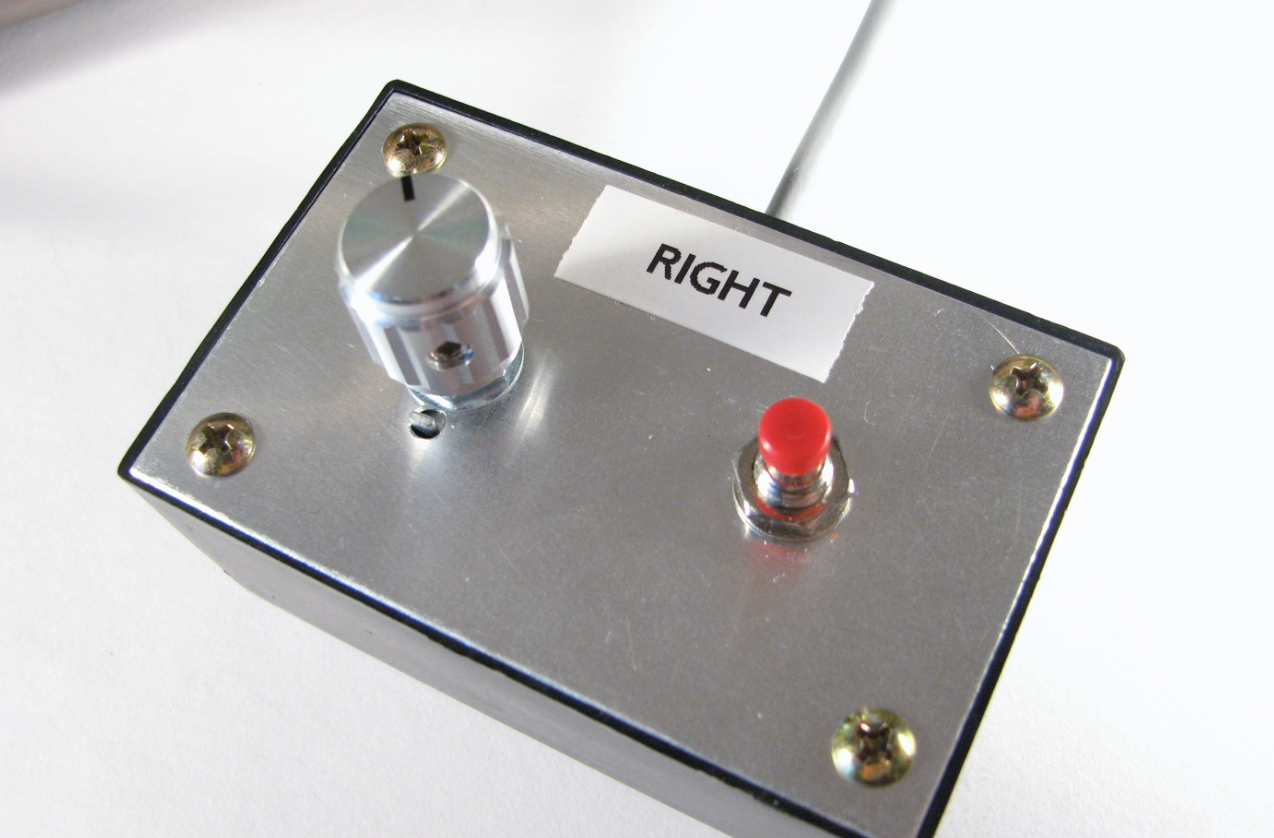
\includegraphics[width=\textwidth/2]{first_controller}
\caption{Replika ovladače pro hru \textit{Tennis for Two}\cite{gamevshardware}}
\end{figure}

\newpage

Větší rozvoj herního hardwaru začal v~roce 1971. Byl vytvořen první herní automat na mince s~hrou \textit{Galaxy Game}. Jednalo se o~hru pro dva hráče ovládanou jednoduchým joystickem. Později se začaly objevovat další automaty a~využívat jak tlačítka, tak i~joystick nebo volant. Hry se v~této době vyskytovaly především na herních konzolích. Vzhledem k~narůstajícím prodejům osobních PC se však začaly dostávat i~do této oblasti, kde byla nejrozsířenejší periferií klávesnice. Vývoj konzolí se však nezastavil.

Převrat v~ovládání PC, a~to i~v~herním průmyslu, způsobil příchod počítačové myši, jak ji známe dnes. Mnoho herních konceptů bylo vylepšeno a~pro hráče to představovalo větší pohodlí během hraní. Kromě toho se vyvíjely alternativní typy ovládání, některé úzce spojeny s~herním žánrem (joystick, volant), nebo naopak vhodné pro mnoho typů her (gamepad)~\cite{gamevshardware}.

Kromě klasických ovladačů se objevují také snahy o~přirozenější ovládání pomocí pohybu, tzv. \textit{motion sensing}. Vzniklo proto několik ovladačů a~herních konzolí, z~nichž nejvýznamnější je Microsoft Kinect vzniklý v~roce 2010~\cite{wikicontrollers}. Více se problematice ovládání pohybem věnuje sekce \ref{section:motion_capture}.

V~současné době se využívá mnoho různých typů ovládání. Následující kapitoly budou věnovány těm nejvíce rozšířeným především v~osobních počítačích. Vysvětlím, k~čemu se dají vhodně využít a~jaké mají nedostatky. Následující přehled bude zároveň sloužit jako podklad pro~analýzu v~praktické části práce.

\section{Klávesnice}

Klávesnice představuje nejpoužívanější počítačovou periferii vůbec. Její princip je velmi jednoduchý: každé stisknutí či uvolnění tlačítka způsobí odeslání informace do PC. Je možné detekovat události více tlačítek najednou, čehož využívají klávesové zkratky.

V~herním průmyslu se klávesnice využívá v~drtivé většině herních žánrů: od jednoduchých arkád, přes závody až po strategie. Jsou vhodné, pokud je potřeba rozlišit větší množství vstupů, které reprezentují jednotlivé klávesy.

Klávesnice ale nemusí být vždy ideální volbou. Diskrétní zpracování vstupu (stisknuto, nestisknuto) představuje nepohodlí při ovládání závodní hry: v~zatáčení je zhoršená citlivost, auto buď zatáčí naplno, nebo vůbec. Tento nedostatek se vývojáři snaží řešit postupným natáčením kol, ale ani to není ideální. Při zatočení v~menší zatáčce je nutné přerušovaně uvolňovat klávesu, aby se vytvořila iluze mírně natočeného volantu. V~kombinaci s~myší může být nevýhodou horší dostupnost kláves vzdálenějších od levé ruky.

\section{Myš}

Počítačová myš je druh polohovacího zařízení. Optický či laserový snímač detekuje pohyb myši po podložce a~převede jej na pohyb kurzoru v~obrazovce. Dále bývá myš vybavena několika ovládacími tlačítky.

Při hraní má široké uplatnění tam, kde je využíván klasický kurzor nebo při nutnosti souvislého, ale přesného pohybu jako například otáčení hráče v~FPS hře\footnote{First-person shooter - akční hra zobrazená z~pohledu herní postavy}.

Nevýhodou při používání myši může být jednostranná zátěž. Kvůli pohybu po stole hráči zatěžují ruku s~myší více, než ruku na klávesnici. Při pravidelném hraní může hráč utrpět poškození z opakovaného namáhání~\cite{rsi}.

\section{Gamepad}

Gamepad je čistě herní periferie. Má tvar určený pro použití oběma rukama. Nachází se na něm množství tlačítek a~může být doplněn jedním, nebo dvěma analogovými joysticky. Některé verze nabízejí i~vibrační odezvu. Nejdříve se využíval u~herních konzolí, s~rozvojem osobních PC se však stal i~zde velmi populární. Primární zaměření na hry dělá z~gamepadu vynikající ovladač pro mnoho herních žánrů. Eliminuje problém ergonomie myši a~klávesnice a~všechna tlačítka jsou snadno dostupná. Proto je velmi často využíván.

Z~hlediska intuitivního ovládání gamepad zaostává podobně jako myš s~klávesnicí. Hry jsou s~ním sice dobře ovladatelné, avšak často je nutný trénink pro~zvládnutí složitějších principů ovládání a~tlačítkových kombinací.

\section{Joystick a~volant}

Joystick a~volant představují ovladače pro specifické druhy her. Základní částí joysticku je páka umístěná kolmo v~pohyblivém kloubu. Má nejlepší uplatnění v~leteckých simulátorech, kde náklon páky mění polohu leteckých klapek. Ovládání je intuitivní a~snaží se přiblížit realitě.

Účelem volantu je simulace ovládání závodního vozu. Obvykle je dodáván s~dvěma nebo třemi pedály a~případně řadicí pákou. Vyšší modely mají vibrační odezvu, při vyjetí z~vozovky tak hráč cítí haptickou odezvu.

Joystick a~volant pomáhají věrně simulovat letecké nebo závodní prostředí, pro které jsou určeny. Na rozdíl od předešlých periferií jsou ale použitelné pouze v~úzké oblasti her, proto bývají nenáročnými hráči nahrazovány gamepadem nebo klávesnicí.

\section{Dotyková obrazovka}

Dotyková obrazovka na~osobních počítačích není v~současné době masově využívána. Větší rozšíření má v~oblasti mobilních zařízení, jako jsou mobilní telefony a~tablety, proto se problematice dotykové obrazovky budu více věnovat v~sekci \ref{section:touchscreen}. Některé hry však využívají dotykovou obrazovku jako~náhradu za jiné periferie (např. myš). Záleží pak na~návrhu samotné hry, zda toto ovládání přinese nějaké benefity, či~bude spíše překážkou.

\section{Ovládání pohybem}

Kromě tradičních hardwarových periferií existují další technologie, jak ovládat hry, a~to pomocí přirozeného pohybu. Tyto systémy snímají pozici hráče nebo zařízení a~podle jejich změn vypočítají reakci ve hře. Ovládání bývá snadné na naučení, protože navozuje pocit přirozené reakce na podněty herního prostředí.

V~této kapitole zmíním dvě technologie: ovládání pomocí akcelerometru a~snímání pohybu těla (\textit{motion capture}). Obě tyto technologie rozšiřují možnosti interakce s~elektronickými zařízeními, fungují však na odlišném principu.

\subsection{Akcelerometr}
\label{section:accelerometer}

Akcelerometr je elektromechanická součástka, která měří zrychlení sil ve třech osách. Tyto síly mohou být statické, jako například tíhová síla, nebo dynamické: způsobeny pohybem nebo vibrováním akcelerometru.\cite{acc} Akcelerometr umožňuje detekovat natočení zařízení v~prostoru a~jeho přibližný pohyb.

V~herním průmyslu se využívá především v~mobilních zařízeních a~v~herních konzolích. Může nahradit joystick, emulovat volant nebo polohovací zařízení. Při využívání akcelerometru může v~nevhodném prostředí docházet k~rušení: například při jízdě v~autobuse je téměř nemožné hrát závodní hru, jelikož při zatáčení autobusu je síla působící na akcelerometr vychýlená a~dochází k~nechtěnému zatáčení.

Další informace o~pohybovém senzoru jsou uvedeny v~sekci \ref{section:accelerometer}.

\subsection{Motion capture}
\label{section:motion_capture}

Velmi zajímavou technologií je ovládání pohybem, tzv. \textit{motion capture}. Jedná se o~snímání části nebo celého těla a~jeho převod v~reálném čase na digitální model. Ten se využívá mimo jiné k~ovládání hry. Nejvýraznějším ovladačem v~herním průmyslu se stal \textit{Kinect} vyvinutý v~roce 2009 firmou Microsoft. \cite{meetthekinect}

\textit{Motion capture} se hodí například pro sportovní nebo akční hry a~to i~při více hráčích. Nevýhodou může být nutnost poměrně velkého prostoru pro potřeby hraní.

\section{Srovnání}

V~minulých kapitolách jsem stručně popsal několik způsobů, jakými lze ovládat hry. Každý z nich má řadu výhod i~nevýhod. Následující tabulka obsahuje shrnutí těchto ovladačů a~porovnání jejich možností. Vzhledem k~tématu této práce se zde budu zabývat především tím, jak je daný způsob interaktivní a~zda tak může obohatit zážitek ze hry.

\begin{table}[h]
\caption{Srovnání herních ovladačů}
\begin{tabularx}{\textwidth}{|l|X|X|}
\hline
\textbf{Ovladač} & \textbf{Výhody} & \textbf{Nevýhody} \\ \hline
Klávesnice & - počet kláves \newline - široké využití & - pouze dva stavy tlačítka (stisknuto, nestisknuto) \newline - některé klávesy hůře dos\-tup\-né \\ \hline
Myš & - přesnost & - jednostranná zátěž \\ \hline
Gamepad & - ergonomický \newline - navržen pouze pro~hry \newline - interaktivní vibrační o\-dez\-va & - ovládání není in\-tui\-tiv\-ní, je třeba se jej naučit \\ \hline
Joystick, volant & - věrně simuluje realitu \newline - interaktivní vibrační o\-dez\-va & - vhodné jen pro některé herní žánry \\ \hline
Dotyková obrazovka & - široké využití \newline - provázanost grafiky s~o\-vlá\-dá\-ním & - v~některých hrách ne\-úspěšně simuluje jiné periferie \\ \hline
Akcelerometr & - intuitivní & - rušení např. v~dopravním prostředku či při jiném pohybu \\ \hline
Motion capture & - velmi přirozené o\-vlá\-dá\-ní & - potřeba většího pros\-to\-ru \\ \hline

\end{tabularx}
\end{table}

\section{Shrnutí}

Srovnání ukazuje rozdíly ovladačů v ergonomii, možnostech zadávání vstupu a dalších parametrech. Pro návrh hry je tak nutné citlivě navrhnout způsob ovládáním a minimalizovat negativní dopady periferií. 

\chapter{Interaktivní prvky v~mobilních telefonech}

V~následující Kapitole 2 se budu věnovat analýze senzorů v~mobilních telefonech, které interagují s~okolním prostředím. Popíšu jejich princip fungování a~využití jak v~mobilních hrách, tak jako interaktivní ovladač počítačové hry. Některé z~těchto senzorů využiji při tvorbě interaktivního ovladače v~Kapitole~\ref{chapter:implementation}.

\section{Dotykový displej}
\label{section:touchscreen}

Dotykový displej je označení pro kombinaci zobrazovacího displeje a~průhledné vrstvy schopné zaznamenávat dotyky vnějších těles, obvykle prstu nebo stylusu. Existuje několik technologií snímání dotyku, stručně popíšu \emph{kapacitní dotykový panel}.

Kapacitní dotykový panel využívá elektrické vodivosti vnějších těles. Dotyk takového tělesa s~povrchem displeje naruší elektrostatické pole obrazovky. Ze změny pole je zjištěno umístění dotyku, které pak dále zpracuje řadič. Kapacitní displeje proto fungují pouze s~vodivými předměty, jako je lidský prst nebo speciální stylus. \cite{gray2013does}

Dotykové displeje nabízejí velmi široké možnosti uplatnění ve hrách. Na rozdíl od klasických ovladačů totiž propojují zobrazení grafiky se samotným ovládáním. Například přesun objektů v~herním světě je velmi přirozený: hráč se jednoduše dotkne objektu a~tahem prstu jej přesune po obrazovce. Ve srovnání s~počítačovou myší odpadá \emph{mezivrstva} ve formě periferie připojené k~zařízení a~hráčův prst se tak stává samotným kurzorem.

Schopnosti dotykových displejů, jako jsou gesta a~snímání více dotyků najednou, zásadním způsobem zjednodušují ovládání mobilních telefonů a~tedy i~mobilních her. Některé jsou přímo postaveny na využití dotykových displejů, např. úspěšná hra \textit{Fruit Ninja}\cite{fruitninja}. Hlavní ovládací prvek představuje tah prstem, který simuluje seknutí čepelí. Hráč se snaží prstem přeseknout co největší množství padajícího ovoce najednou. Hra je příkladnou ukázkou využití dotykové obrazovky: letící ovoce představuje podnět, aby se hráč trefil do daného místa na obrazovce. Ovládání tak přímo koresponduje se zobrazovanou grafikou (pokaždé je pro optimální přeseknutí potřeba jiné gesto prstem) a~splývá s~hrou v~jednu ucelenou část.

\begin{figure}
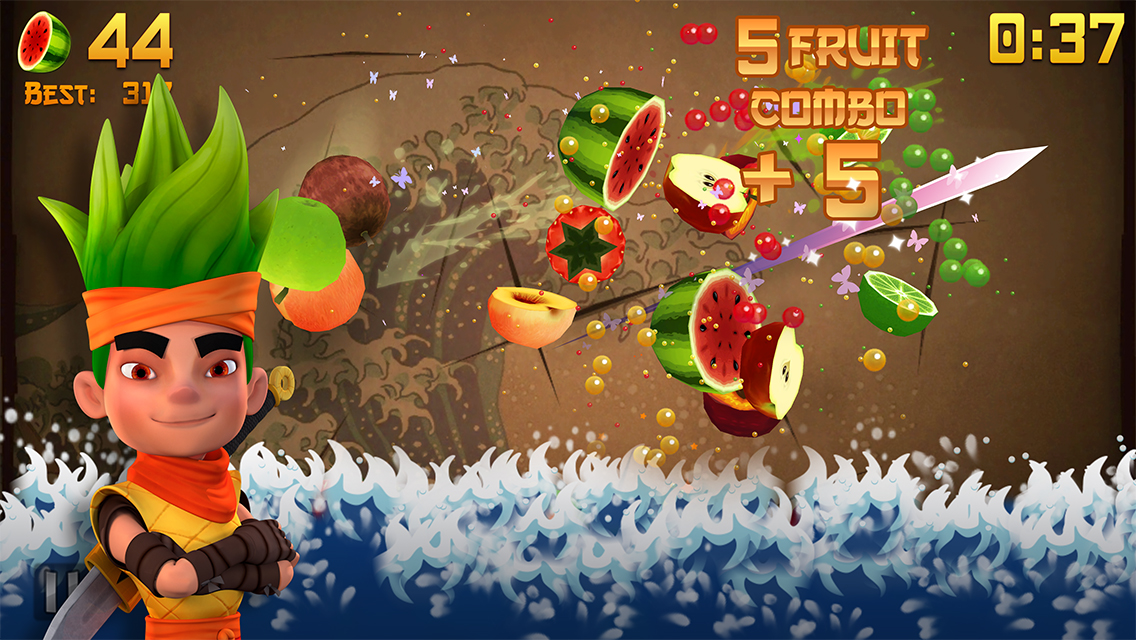
\includegraphics[width=\textwidth]{fruit_ninja}
\caption{Využití dotykové obrazovky ve hře Fruit ninja\cite{fruitninja}}
\end{figure}

Této provázanosti se dá využít i~v~počítačové hře ovládané mobilním telefonem: Hlavní herní scéna je zobrazována na displeji počítače a~hráč drží v~ruce ovladač (mobilní telefon), který je spojen s~hrou v~PC. Dotyková obrazovka zde může plnit funkci jak ovládací, tak i~zobrazovací. To nemusí být nutně výhodou, protože při ovládání hry se hráč přirozeně soustředí především na obraz v~PC a~může být nepohodlné často měnit pohled z~monitoru na mobil. Pokud je ale hra určena pro více hráčů, otevírají se nové možnosti, jak využít individuální obrazovku každého hráče: informace na mobilním displeji mohou například tvořit herní výhodu pro jednotlivé hráče.

Této techniky lze však dosáhnout pouze úzkým provázáním hry s~ovladačem. Vzhledem k~těmto schopnostem mobilních telefonů v~kombinaci s~dostatečným výkonem, dalšími senzory a~rychlou bezdrátovou komunikací má využití dotykového displeje velký potenciál.

Kromě interaktivní provázanosti může být dotyková obrazovka využita jako vstupní zařízení ve~formě klasických dotykových tlačítek či pro detekci gest jedním nebo více prsty.

\section{Akcelerometr}
\label{section:accelerometer}

Dalším interaktivním senzorem je akcelerometr. Objevuje se v~ovladačích k~herním konzolím i~v~mobilních telefonech, kde plní různé funkce: zajišťuje automatickou orientaci displeje v~závislosti na natočení mobilu, pohybová gesta jako například zatřesení nebo položení displejem dolů mohou sloužit k~ovládání systému a~široké využití má ve hrách.

Existuje velké množství mobilních her využívající náklon telefonu k~ovládání. Následující výčet obsahuje přehled častých použití. Každý příklad doplňují hry, kde se tyto prvky vyskytují: \cite{accelerometergames}:

\begin{itemize}
	\item Simulace volantu v~závodní hře (Lane Splitter, Jet Car Stunts)
	\item Náklon telefonu odpovídá náklonu herní podložky (Crazy Labyrinth 3D)
	\item Využití akcelerometru jako joysticku v~leteckém simulátoru (Skies of Glory)
	\item Náklon telefonu mění pozici herního objektu (Donkey Jump, Box Busters)
\end{itemize}

Pro interaktivní ovladač k~PC hře je použití akcelerometru ideální příležitostí. Pohyb herního objektu náklonem telefonu je pro člověka přirozenější a~vtahuje hráče intenzivněji než ovládání tlačítky. 

\section{Gyroskop}

Gyroskop je součástka pro detekci polohy zařízení. Měří změnu úhlu natočení telefonu kolem své osy. To umožňuje detekovat pohyb zařízení lépe než akcelerometr, ale vzhledem k~detekci relativní změny se postupem času objevuje odchylka, a~proto se gyroskop využívá v~kombinaci s~akcelerometrem a~někdy též s~kompasem. Díky tomu je možné určit natočení telefonu vůči gravitační síle a~detekovat změnu polohy zařízení ve všech směrech. \cite{gyroscope}

\section{Senzor přiblížení}

Senzor přiblížení, nebo také \textit{proximity senzor}, funguje na principu detekce elektromagnetického záření, které generuje vysílač. V~případě přiblížení objektu do blízkosti snímače je zaznamenán odraz záření zpět k~senzoru a~je vyhodnocena vzdálenost objektu. \cite{proximity}

Nejběžnější využití proximity senzoru v~mobilním telefonu je při hovoru. Před přiložením k~uchu senzor detekuje přiblížení hlavy a~zhasne displej. Zabrání tím tak nechtěnému ukončení hovoru dotykem ucha s~obrazovkou.

Herní využití proximity senzoru není obvyklé, neexistují žádné hry využívající proximity senzor ve hře, pouze simulace tlačítka v~PC hře podomácku vyrobeným senzorem přiblížení. \cite{proximitygame}

\section{Ostatní senzory}

Současné mobilní telefony mohou disponovat ještě několika dalšími senzory okolního prostředí, ale vzhledem k~minimálnímu využití v~herní oblasti zde nebudou více zkoumány. Jedná se například o~senzor okolního světla, teploměr a~magnetický senzor (kompas). 

\section{Shrnutí}

V~této kapitole byly popsány nejčastější interaktivní senzory vyskytující se v~dnešních mobilních telefonech, jejich princip a~možné využití. V~kapitole \ref{chapter:implementation} se budu snažit některé z~nich využít při tvorbě interaktivního ovladače pro PC hru. 

\chapter{Podobná řešení}

Před samotnou tvorbou softwarového projektu zmíním podobné systémy na trhu. V~současné době již existují řešení využívající mobilní telefon k~ovládání jiné hry. Každé z~nich však obsahuje nedostatky a~narušuje tak výsledný zážitek.

\section{Telefon jako univerzální gamepad}

Na internetu existuje velké množství aplikací, které nabízejí funkcionalitu podobnou bezdrátovému gamepadu. Ukázkou takové aplikace je např. Mobile Gamepad \cite{mobilegamepad} Po nainstalování příslušného ovladače do PC je možné využít telefon jako vstupní zařízení: umožňuje nastavit si tlačítka na displeji, pohybový senzor jako joystick atd.

\begin{figure}[h]
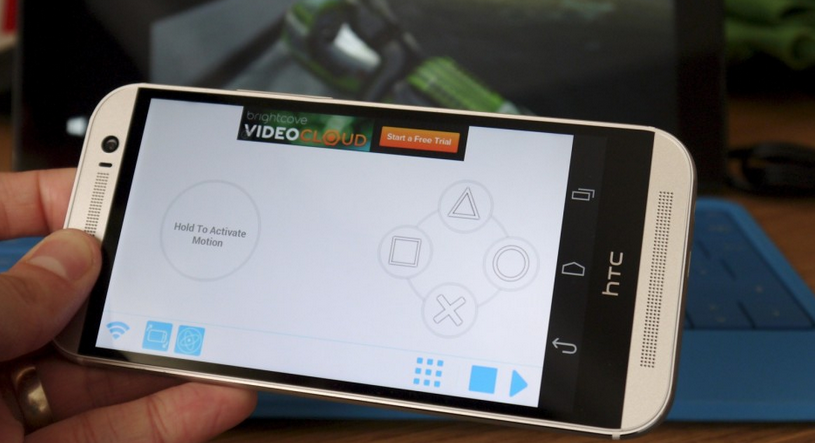
\includegraphics[width=\textwidth]{mobile_gamepad}
\caption{Mobilní telefon jako univerzální gamepad\cite{mobilegamepad}}
\end{figure}

Výhodou tohoto řešení je možnost ovládat PC podobně jako jiné ovládací periferie a~díky tomu není ovladač vázán na konkrétní hru. Co však brání použití v~interaktivní hře, je absence jiných funkcí než těch, které již obsahují gamepady a~podobné ovládací prvky. To je způsobeno univerzálností ovladače. Pro zachování standardizovaného ovládacího rozhraní a~chování jako klasické vstupní zařízení počítače není umožněna širší komunikace s~hrou. Tyto aplikace tak nabízejí stejnou nebo často i~méně kvalitnější alternativu ke klasickým herním gamepadům a~jiným ovladačům. 

\section{Apple AirPlay}

Společnost Apple nabízí pro své telefony funkci sdílení obrazu na externí obrazovku. Toho je docíleno pomocí zařízení AppleTV a~bezdrátové technologie AirPlay\cite{airplay}.

Toto řešení již lépe využívá interaktivní možnosti mobilních přístrojů, integrovaný displej tvoří druhou obrazovku, může zobrazovat ovládání dobře optimalizované pro konkrétní hru nebo dodatečné informace o~hře (skóre, počet ujetých kol atd.). Zásadní nevýhodou však je nemožnost hrát hru s~více hráči kvůli zvolené architektuře: herní logika včetně vykreslování běží na straně mobilního zařízení a~do externí obrazovky se přenáší pouze obraz.

\begin{figure}[h]
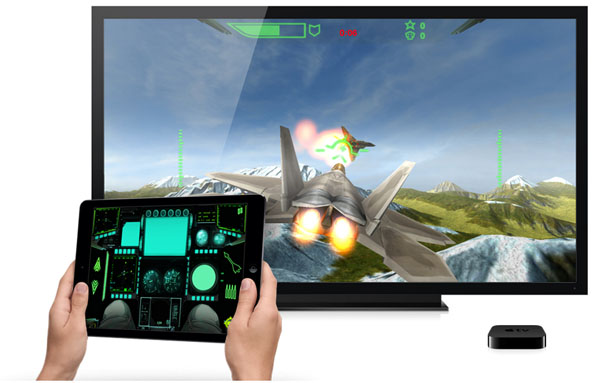
\includegraphics[width=\textwidth]{airplay}
\caption{Technologie AirPlay\cite{airplay}}
\end{figure}


\section{AirConsole}

Řešením, které se nejvíce podobá tématu této bakalářské práce, je herní platforma švýcarského startupu AirConsole\cite{airconsole}. Jedná se o~webovou aplikaci společně s~multiplatformní mobilní aplikací. Pomocí webového prohlížeče se vytvoří hra a~k~ní se připojí telefony jako ovladače. V~nabídce je několik různých her a~každá má vlastní ovladač v~rámci mobilní aplikace. Samotná hra tedy probíhá na obrazovce počítače. AirConsole také poskytuje API, takže lze vytvořit vlastní hru v~HTML5 nebo herním enginu Unity a~propojit ji s~tímto systémem.

\begin{figure}[h]
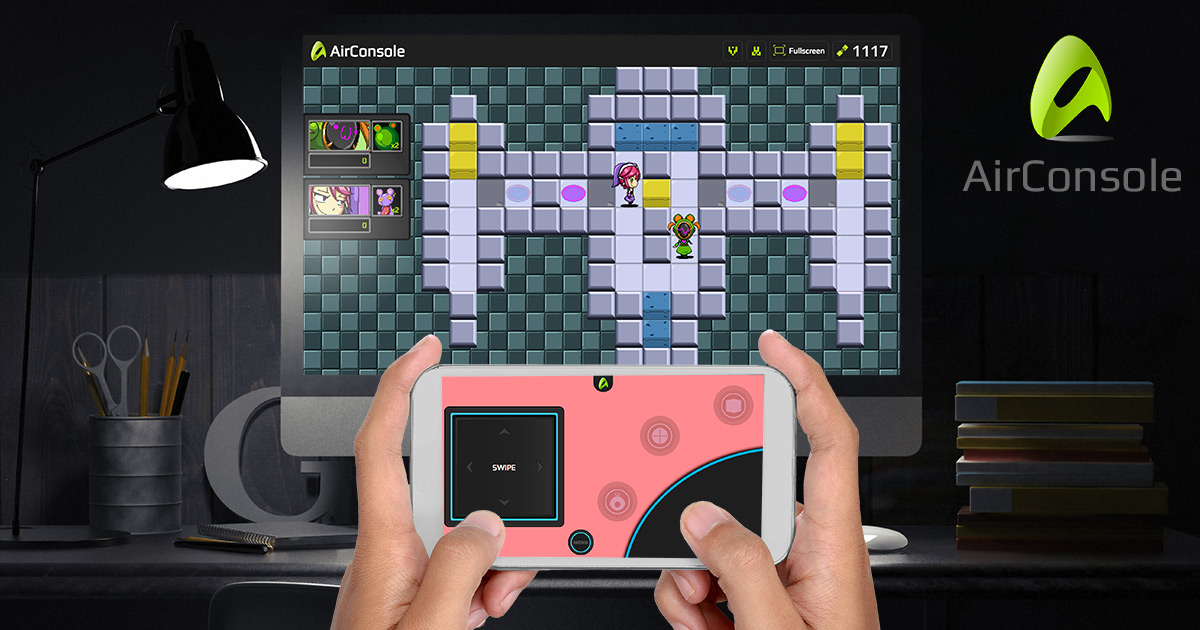
\includegraphics[width=\textwidth]{airconsole}
\caption{Ukázka hry pomocí systému AirConsole\cite{airconsole}}
\end{figure}

Spojení probíhá přes externí servery, konkrétně přes infrastrukturu Google\cite{airconsole}. Kvůli tomu, že telefony nekomunikují s počítačem přímo, ale přes servery společnosti Google, má spojení větší odezvu, což silně ovlivňuje zážitek ze hry. Ovládací rozhraní je vytvořené pomocí HTML5, na displeji se tedy vykresluje webová vrstva. Zpracování dotyku v~tomto případě není ideální, objevují se chyby (například špatná detekce kliknutí) a~projevuje se vyšší odezva. Zároveň ovládání nevyužívá interaktivní možnosti mobilních telefonů, jediný možný způsob interakce je pomocí dotykového displeje. AirConsole tak vytváří podobnou funkcionalitu, jako je emulace gamepadu.

Přes všechny tyto nedostatky se AirConsole nejvíce blíží zaměření této práce, především hlavním cílem, a~to vytvořit herní platformu podporující mezilidskou komunikaci lidí fyzicky přítomných na jednom místě.

\section{Možnosti řešení}

V~rámci této práce jsem nalezl tři možnosti řešení, jak odstranit nedostatky předchozích systémů:

\subsection{Rozšíření existující PC hry}

Prvním způsobem vytvoření ovládání pomocí mobilního telefonu je vytvoření mobilního ovladače k~již existující PC hře s~otevřeným zdrojovým kódem. Stěžejní částí by bylo vytvoření „adaptéru“ napojeného na mobilní telefon. Nevýhodou je rozsáhlost takového projektu a~složitost jejího rozšíření o~interaktivní prvky.

\subsection{Univerzální herní ovladač}

Druhým způsobem je vytvoření mobilní aplikace poskytující rozhraní pro komunikaci s~libovolnou hrou. Podobně je vytvořen systém AirConsole. Jeho velkou výhodou je univerzálnost použití, kdy jedna mobilní aplikace může být využita pro~mnoho her, které implementují požadované rozhraní. Na rozdíl od AirConsole by pro univerzální použití včetně interaktivních senzorů muselo rozhraní podporovat velké množství funkcí, např. definice ovládání, načtení grafiky z~libovolné hry, poskytnutí ovládací logiky mobilnímu ovladači a~funkce pro využití mobilních senzorů. Složitost tohoto řešení však překračuje rozsah bakalářské práce.

\subsection{Komunikační modul}

Třetí možností je vytvoření systému pro síťovou komunikaci PC a~ovladače. Takovéto řešení by bylo možné použít při vývoji libovolné hry, ale s~nutností vytvořit samostatný ovladač zvlášť pro každou hru. Na druhou stranu není třeba vytvářet rozhraní pro sdílení herní logiky a~grafických prvků, to může být implementováno v~ovladači nebo vyřešeno sdílením zdrojového kódu s~hrou. Zařízení si budou mezi sebou posílat zprávy s~herními informacemi, na které budou reagovat definovaným způsobem. Tento návrh umožňuje vytvořit snadno integrovatelný systém komunikace. Mobilní telefony budou mít zároveň širší možnosti využití hardwaru.

Toto řešení jsem zvolil pro implemetaci v~bakalářské práci, protože eliminuje nevýhody stávajících řešení na trhu a~zároveň nabízí přijatelný kompromis mezi složitostí systému a~univerzálností pro případ použití v~dalších hrách. 

\chapter{Tvorba systému}
\label{chapter:implementation}

Informace o~možnostech ovládání hry pomocí mobilního telefonu využiji v~praxi a~vytvořím systém, ve kterém bude mobilní telefon v~roli interaktivního ovladače PC hry. To vyžaduje tvorbu komunikačního protokolu a hry, která bude využívat tento protokol. Softwarový projekt komunikačního protokolu i~hry samotné je hlavní náplní praktické části této bakalářské práce.

Struktura kapitoly odpovídá vývojovým fázím softwarového projektu. \cite{si} První část je zaměřena na~analýzu systému, požadavky a~softwarový návrh, v~implementační fázi zmíním některé zásadní části realizace, testování programu a~hratelnosti a~na závěr se budu zabývat možnostmi, jak by bylo možné vytvořený systém rozšířit v~budoucnosti.

\section{Požadavky}
\label{section:requirements}

Cílem první fáze softwarového projektu je specifikace vlastností projektu, určení prostředí, ve kterém bude systém nasazen, a~vymezení funkcionalit nutných pro naplnění účelu systému.

Pro ucelený přehled o~systému nejprve popíšu běžný průběh hraní hry postavené na systému vytvořeném v~této práci: Skupina hráčů s~chytrými telefony se připojí do jedné WiFi sítě společně s~PC, kde poběží hra (server). Poté spustí ovladač v~mobilním telefonu, který automaticky vyhledá hry dostupné v~lokální síti. Po kliknutí na název nalezené hry naváže ovladač spojení s~hrou. Hráč, který může měnit nastavení hry (\textit{admin}, typicky první připojený hráč), nastaví parametry hry a~po připojení všech hráčů zahájí hru. V~případě odpojení nebo ztráty spojení bude možné se do hry opět připojit. Po skončení hry se systém dostane do stejné fáze jako před jejím zahájením, tj. bude opět možné měnit herní parametry apod.

Z~výše uvedeného scénáře budu vycházet při tvorbě požadavků, které jsou rozděleny do dvou částí: komunikační protokol a~hra samotná. Každá část má vlastní seznam funkčních a~nefunkčních požadavků. Tyto požadavky představují základní kritéria pro~návrh architektury systému a~jeho funkcionalit.

\subsection{Komunikační protokol}

Účelem komunikačního protokolu je zajistit obousměrnou výměnu zpráv mezi mobilním telefonem (\textit{ovladačem}) a~počítačem (\textit{hrou}). K~tomu je vhodné použít stejný systém v~obou zařízeních, aby je bylo možné implementovat pouze jednou a~ne pro každou platformu zvlášť. Stejně tak je třeba zachovat identickou strukturu síťových zpráv mezi všemi zařízeními.

Ovladače budou s~hrou komunikovat v~lokální Wi-Fi síti. Při bezdrátové komunikaci je nutné počítat s~výpadky signálu. Může je způsobovat nedostatečný výkon Wi-Fi routeru, příliš velká vzdálenost od vysílače nebo objekty v~prostoru, které brání šíření signálu. Proto je třeba u~zpráv rozlišit, zda je nutné, aby byla doručena spolehlivě (např. kliknutí hráče na tlačítko), nebo zda systému nevadí případná ztráta zprávy (např. často se opakující informace z~pohybového senzoru). 

Vzhledem k~univerzálnímu zaměření systému je vhodné oddělit přenos zpráv a~jejich zpracování (parsování) pro dosažení větší modularity. Dále je výhodné umožnit  konfiguraci síťových parametrů, aby odpovídala požadavkům konkrétní hry.

Specifikace funkčních požadavků softwarového systému popisuje základní chování systému a~jeho dílčích částí. Tato specifikace slouží jako nutný základ při návrhu projektu a~také jako podklad pro zhodnocení úspěšnosti aplikace. \cite{pozadavky}

Pro komunikační protokol platí tedy následující funkční požadavky:

\begin{enumerate}
	\item Systém umožňuje nalézt všechny běžící hry v~lokální síti.
	\item Každá síťová zpráva má tyto vlastnosti: typ zprávy, data zprávy, spolehlivost doručení, zachování pořadí.
	\item Hra i~ovladač dokážou detekovat ztrátu spojení.
	\item Síťový port (nebo jejich rozsah) a~další lze definovat zvlášť jak pro ovladač, tak pro hru.
	\item Ovladač umožňuje odeslání informací o~interakci uživatele (kliknutí na tlačítko, data z~pohybového senzoru).
	\item Ovladač je schopen přijímat informace o~stavu hry (herní události, kompletní stav hry pro vykreslení na mobilním displeji).
\end{enumerate}

Funkční požadavky jsou doplněny požadavky nefunkčními, které specifikují kvalitu aplikace podle kritérií. Mezi ně se řadí například výkon, spolehlivost, rozšiřitelnost a~další. Zaměřil jsem se především na cílovou platformu, modulárnost a~jednoduché nasazení v~dalších hrách:

\begin{enumerate}
	\item Síťová komunikace probíhá v~rámci stejné Wi-Fi sítě. Podpora pro \textit{blue\-tooth} a~další bezdrátové technologie není implementována.
	\item Komunikační systém běží na alespoň jedné mobilní platformě (Android, iOS nebo Windows Phone) a~alespoň jedné PC platformě (Windows, Linux nebo OS X).
	\item Systém je modulární: je možné definovat vlastní typy zpráv, jejich strukturu a~vlastnosti podle požadavků hry.
	\item Parsování zpráv nezávisí na komunikačním frameworku. Je možné implementovat rozdílné parsování nebo i~několik různých metodik najednou.
	\item Zdrojový kód komunikačního modulu je sdílený mezi hrou a~ovladačem.
	\item Komunikační modul nezávisí na herním engine a~herním žánru, a~je tak použitelný v~libovolné hře.
\end{enumerate}

\subsection{Hra}

Požadavky na hru a herní zařízení se v~první řadě netýkají žánru a~obsahu, ale snaží se především využít komunikační systém a~možnosti interaktivity. Volba žánru a~konkrétního typu hry je proto přesunuta až do fáze návrhu, kde bude nutné vhodně navrhnout zapracování interaktivních prvků do herních mechanik.

Důležitou vlastností hry je demonstrace nových možností oproti klasickým ovladačům. Mezi ně se mimo jiné řadí schopnost vykreslování grafiky v~mobilní obrazovce. Tuto a~další nové možnosti je třeba ve hře 
výrazně prezentovat.

Pro celou hru (ovladač i~PC) platí následující funkční požadavky:

\begin{enumerate}
	\item Hra využívá k~ovládání pohybový senzor mobilního telefonu a~dotykovou obrazovku.
	\item Ovladač je schopen vykreslit herní scénu nebo její část na obrazovce mobilního telefonu.
	\item Hra je určena pro 2 až 8\footnote{Více hráčů již není praktické pro zobrazení na jedné obrazovce.} hráčů (ovladačů).
	\item Mobilní telefon může využívat vibrace jako interaktivní odezvu na události ve hře.
 	\item Každá instance hry má nastaven název serveru a~herní parametry.
	\item Parametry hry může měnit právě jeden z~připojených hráčů.
	\item Zvolený herní žánr je vhodný pro hru více hráčů a~obsahuje jak kooperativní, tak kompetitivní složku.
	\item Veškerá konfigurace hry probíhá pomocí ovladače: po spuštění hry na PC již není potřeba další obsluha PC (mimo ukončení hry).
	\item Zobrazováním hry nebo její části na displeji mobilního telefonu přináší danému hráči taktickou výhodu oproti ostatním.

\end{enumerate}

Nefunkční požadavky na hru zahrnují především použití cílové platformy:

\begin{enumerate}
	\item Ovladač poběží na alespoň jedné mobilní platformě (Android, iOS nebo Windows Phone).
	\item Hra poběží alespoň na jedné PC platformě (Windows, Linux nebo OS~X).
	\item Použitý herní engine je multiplatformní a~použitelný jak ve hře, tak v~ovladači.
\end{enumerate}

\section{Návrh}

Návrh systému je druhou fází softwarového projektu. Obsahuje podrobnější popis komponent systému, jejich objektů a~popis jejich vzájemných vztahů.

Hra pro PC i~ovladač používají dvě základní komponenty. První z~nich je síťový modul zajišťující veškerou síťovou komunikaci a~druhou komponentou je herní engine. 

\subsection{Komunikační modul}

Úkolem komunikačního modulu je zajistit výměnu zpráv v~lokální síti. Kromě toho definuje obecnou síťovou zprávu a~její vlastnosti. Modul tedy tvoří dvě základní komponenty: \code{Box} a~\code{Connector}. 

Hlavním přínosem modulu je odstínění implementace síťové vrstvy od hry a~herního enginu a~velmi snadné nasazení v~libovolné jiné hře zaměřené nejen na interaktivní ovládání pomocí mobilního telefonu. Výhodou vytvoření abstraktní vrstvy v~porovnání s~přímým použitím RakNetu je především zjednodušení navázání spojení, manipulace s~datovými pakety a~nezávislost na vnitřní implementaci.

\begin{figure}[h]
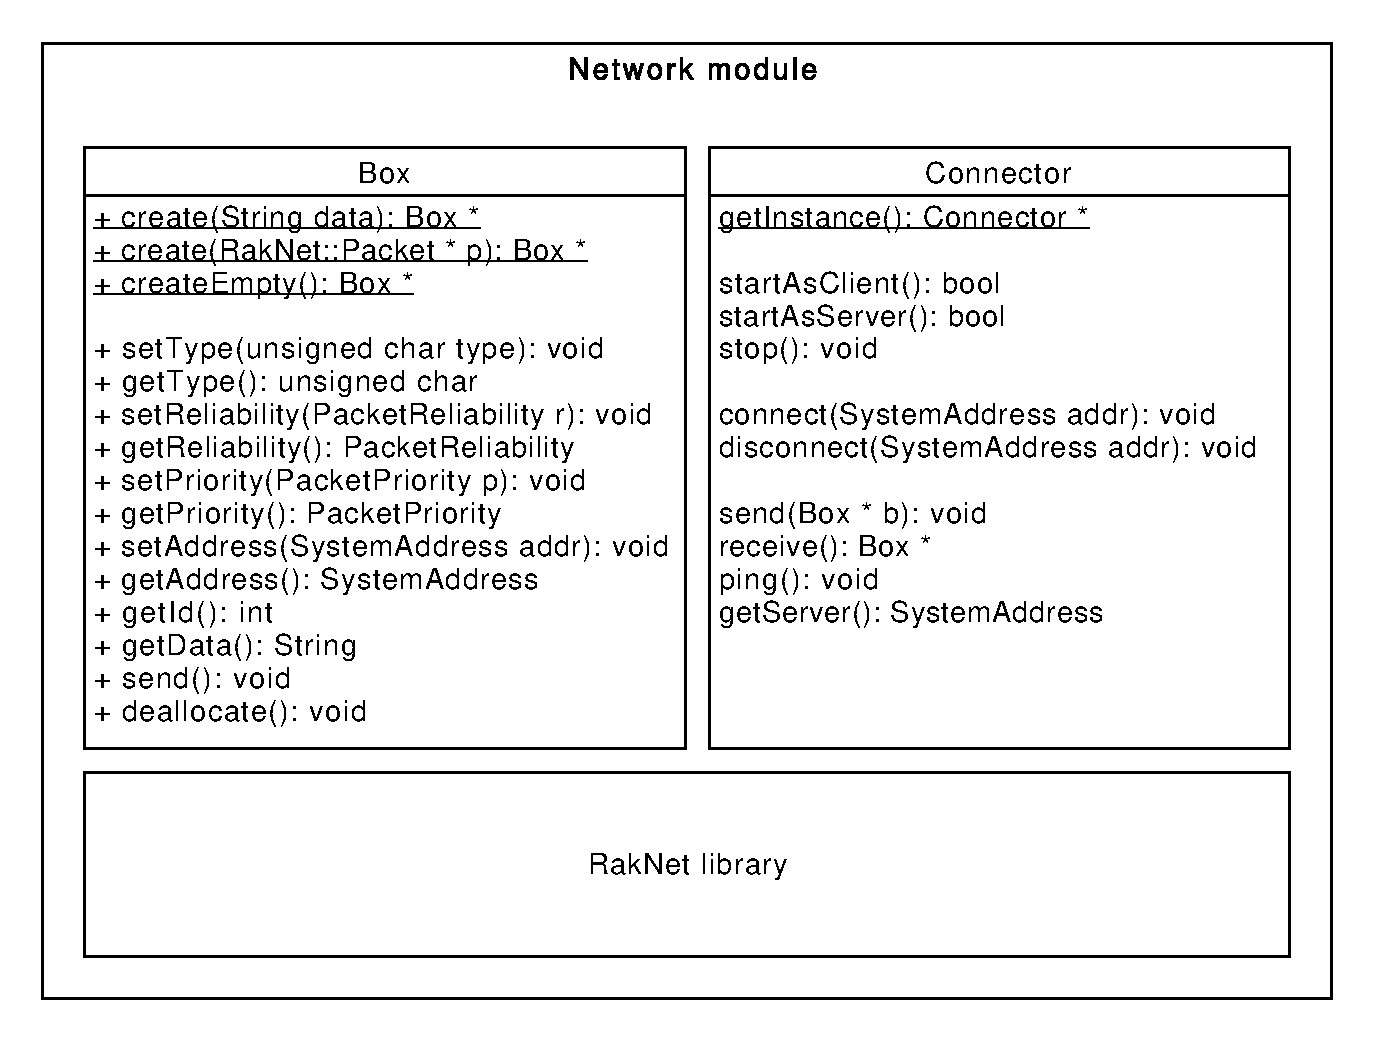
\includegraphics[width=\textwidth]{box_connector}
\caption{Struktura síťového modulu}
\end{figure}

\subsubsection{Box}

\code{Box} je objekt reprezentující síťovou zprávu. Používá se jako vyšší úroveň abstrakce pro předávání herních zpráv mezi klienty a serverem. Jeho cílem je zapouzdřit veškeré informace potřebné pro práci s daty. Používá se v~obou směrech komunikace, což znamená, že se vytváří před odesláním, ale také po přijetí zprávy.

Obsahuje data zprávy, typ zprávy, adresu příjemce (pokud bude zpráva odeslána), nebo adresu odesílatele (pokud byla zpráva přijata), dále vlastnosti doručení, mezi které patří spolehlivost (spolehlivé doručení znamená, že odesílající zařízení čeká na potvrzení přijetí zprávy), priorita, jak rychle má být zpráva doručena (zprávy s~nízkou prioritou mohou být řazeny do fronty a~odeslány najednou, což šetří síťový provoz) a~nastavení, zda je nutné dbát na zachování pořadí zpráv, v~jakém byly odeslány.

\subsubsection{Connector}

\code{Connector} je objekt, který stanovuje programové rozhraní veškerého fungování síťové komunikace: obsahuje metody pro aktivování síťových rozhraní, připojování a~odpojování klientů, posílání a~příjem zpráv. Společně se třídou \code{Box} tvoří základní pilíř pro výměnu zpráv mezi hrou a~ovladačem.

\subsubsection{RakNet}

Hlavičková definice tříd \code{Connector} i~\code{Box} tvoří abstraktní rozhraní nad samotnou implementací a~umožňuje tak snadnou změnu platformy, případně síťové knihovny. Pro implementaci rozhraní jsem zvolil knihovnu RakNet.

RakNet je multiplatformní síťová knihovna se zaměřením na hry. Je napsaná v~jazyce C++. Vyznačuje se velmi nízkými nároky na hardware, kvalitní dokumentací a~množstvím funkcionalit, které se často využívají v~multiplayerových hrách. \cite{raknet} Mezi ně patří například Lobby systém\footnote{Lobby systém - virtuální místnost, kde se shromažďují hráči před začátkem online hry. Obvykle nabízí chat mezi hráči, volbu herních místností nebo žebříček výsledků.}, šifrování komunikace nebo peer-to-peer spojení mezi hráči. Veškerá komunikace je postavena na protokolu UDP, přesto knihovna obsahuje vlastní implementaci pro podporu spolehlivého doručení zpráv.

Knihovnu jsem zvolil především pro její snadné použití, kvalitní dokumentaci a~podporu jak klasických počítačů, tak i~mobilních platforem. Stejnou implementaci modulu je tak možné využít v~ovladači i~ve hře na PC.

\subsection{Hra}

Návrh hry se skládá z~několika částí. Prvním krokem je volba herního žánru. Poté se budu věnovat hledání herního enginu, na kterém bude hra postavena. Poslední částí bude již samotný návrh struktury systému, objektů, vztahů mezi nimi a~tvorba samotného komunikačního protokolu.

\subsubsection{Volba herního žánru}

Jak bylo zmíněno v~analýze, důležitým požadavkem pro hru je možnost efektního využití interaktivních možností chytrých telefonů. K~tomu musí být uzpůsoben herní žánr tvořící kostru veškeré hratelnosti. Proto jsem nejprve zvolil dva směry a~porovnával jejich výhody a~nevýhody:

Prvním z~nich je akční 2D hra, kde kamera zobrazuje scénu shora. Hlavním pilířem hry je souboj dvou týmů. Cílem je dosáhnout většího počtu zásahů než protivník. Každý hráč ovládá jednu postavu vybavenou zbraní. Mezi interaktivní prvky lze zařadit ovládání postavy pohybovým senzorem a~intuitivní míření pomocí dotykového displeje (místo dotyku prstu a~střed obrazovky vytvoří přímku definující směr výstřelu). Inovativním prvkem je zobrazení herní mapy: většina herního území se zobrazuje na obrazovce, kterou vidí všichni hráči. Vyskytují se ale místa, kde hráč může vyjít mimo herní území (např. dveře nebo vchod do domu). Po vkročení na tato místa postava zmizí z~hlavní obrazovky a~danému hráči se na mobilním displeji vykreslí interiér domu i~s~hráčem. Tímto se elegantně rozšíří herní prostor na další objekty a~zároveň je zachována interaktivita mezi hráči (např. je možné zasáhnout hráče v~domě skrz okno). Zmíněný prvek považuji za velmi efektní příklad využití mobilního telefonu, který obohacuje samotnou hru a~přináší nové taktické možnosti.

Tento návrh hry bohužel obsahuje i~méně vhodné prvky. Zobrazení velké části mapy, kterou uvidí hráči obou týmů, odhaluje pozice všech hráčů a~ubírá tak možnost taktizování v~terénu, jelikož se hráč nemůže skrýt před protivníky jinak, než že vejde do výše zmiňované \uv{interaktivní místnosti}. Tím by však mohla nastat situace, že hráči budou takto skrytí příliš často a~hlavní obrazovka téměř ztratí význam.

Druhým návrhem je sportovní zaměření, konkrétně 2D fotbal. Podobně jako u~akční hry má kamera pohled shora a~soupeří proti sobě dva týmy s~cílem skórovat vícekrát než soupeř. Hlavní obrazovka zobrazuje fotbalové hřiště s~hráči. Hráč ovládá svou postavu pomocí akcelerometru a~dotyk s~obrazovkou mu umožňuje vystřelit (sílu výstřelu určuje doba dotyku před uvolněním prstu z~obrazovky). Obohacením hry jsou bonusy. Objevují se náhodně na hřišti a~při jejich sebrání poskytuje danému hráči časově omezenou výhodu. Mezi bonusy patří zvýšení rychlosti, zvětšení maximální síly kopu a~především neviditelnost. Neviditelný hráč zmizí z~hlavní obrazovky a~na mobilním displeji se mu začne vykreslovat hřiště totožné s~hlavní obrazovkou. Jeho taktická výhoda spočívá v~tom, že sám sebe vidí, ale není viděn ostatními a~může procházet skrz hráče. Bonus neviditelnosti představuje výraznou inovaci podobně jako rozšířené místnosti v~návrhu akční hry, eliminuje však případné nedostatečné využití hlavního displeje.

Všechny zmíněné a~ještě některé další výhody a~nevýhody těchto dvou návrhů shrnuje tabulka \ref{table:game_comparison} (prvek s~větším přínosem je vyznačen kurzivou).

\begin{table}[h]
\caption{Srovnání vybraných herních žánrů}
\label{table:game_comparison}
\begin{tabularx}{\textwidth}{|X|X|}
\hline
\textbf{Akční hra} & \textbf{Fotbal} \\ \hline
\multicolumn{2}{|c|}{Pohyb postavy pomocí akcelerometru}\\ \hline
\multicolumn{2}{|c|}{Taktická výhoda při zobrazení hry v~mobilním displeji}\\ \hline
\multicolumn{2}{|c|}{Obsahuje kooperativní i~kompetitivní složku hry}\\ \hline
% & \\ \hline
\emph{Rozšíření scény o~interaktivní místnosti} & Bonus neviditelnosti \\ \hline
Riziko časté nepřítomnosti na hlavní obrazovce & \emph{Možnost neviditelnosti je časově omezena} \\ \hline
Hlavní obrazovka ubírá možnosti taktizování & \emph{Hřiště je optimální pro zobrazení na společné obrazovce} \\ \hline

Střelba na základě místa dotyku s~obrazovkou & Síla kopu se odvíjí od délky dotyku \\ \hline
Míření může být těžké na naučení & \emph{Kopnutí je velmi intuitivní} \\ \hline
% & \emph{} \\ \hline
\end{tabularx}
\end{table}

Podle tabulky se jeví jako vhodnější kandidát implementace fotbalu. Mě osobně více zaujal i~z~důvodu atraktivity pro diváky například na večírku s~přáteli, kteří mohou být jako pozorovatelé lépe začleněni do hry. 

Po zvážení všech těchto aspektů jsem se rozhodl použít fotbal jako téma demonstrační hry.

\subsection{Herní engine}

Slovní spojení herní engine je možné definovat různými způsoby. Závisí například na provázanosti herní logiky s~vykreslováním, obecnosti enginu z~pohledu herního žánru apod. V~této práci je pod pojmem \textit{herní engine} myšlen softwarový framework, který obsahuje základní komponenty potřebné pro vývoj her, jako je vykreslování grafiky, detekce kolizí, zpracování uživatelských vstupů, práce se zvukem a~další. \cite{gameengine}

Důležitou částí návrhu je výběr herního enginu. Pro účely této hry jsem stanovil několik požadavků, které musí engine splňovat:

\begin{itemize}
	\item Podpora více platforem (jak PC, tak i~mobilní telefony) podobně jako RakNet, aby bylo možné použít oba tyto frameworky současně. Pokud engine nebude napsán v~jazyce C++, měl by podporovat práci se sítí, nebo musí existovat alternativní síťová knihovna použitelná s~tímto enginem.
	\item Vzhledem k~nulovému finančnímu rozpočtu tohoto projektu musí být engine licencován zdarma.
	\item Herní engine musí umět pracovat s~2D grafikou a~být nezávislý na herním žánru.
	\item Mezi funkce herního enginu musí patřit mimo jiné podpora dotykové obrazovky a~zpracování pohybového senzoru.
	\item Musí existovat volně dostupná kvalitní dokumentace a~návody, jak herní engine používat.
\end{itemize}

Z~velkého množství různých možností se do výběru použitelných enginů dostal \textit{Torque 2D}, \textit{Cocos2d-x} a~\textit{Marmalade}. Všechny tyto enginy nabízejí funkce splňující výše uvedené požadavky. Nevýhodou Torque 2D je méně rozsáhlá dokumentace a~návody v~porovnání s~Cocos2d-x a~Marmalade, proto jsem jej vyřadil. Při rozhodování mezi Cocos2d-x a~Marmalade jsem bral v potaz také licenci na herní engine: Cocos2d-x je na rozdíl od Marmalade zveřejněn s otevřeným zdrojovým kódem, proto jsem jej zvolil pro tuto práci.

\subsection{Návrh ovládání}

Ovládání hry je realizováno pomocí mobilního telefonu spojeného se hrou. Pro připojení do hry a~nastavení parametrů zápasu počítá návrh s~klasickým využitím tlačítek zobrazených na dotykové ploše. Mimo to je třeba navrhnout ovládání akcí herní postavy v~zápase. Tyto akce jsou dvě: pohyb a~kopnutí do míče.

Hlavní ovládací prvek pohybu tvoří akcelerometr. Zajišťuje pohyb herní postavy po dvourozměrné ploše hřiště. Změřením velikosti náklonu telefonu se vypočítá směr a~rychlost hráče. Toto ovládání je zajímavé především z~pohledu křivky učení: je velmi jednoduché pochopit princip pohybu pomocí akcelerometru, ale získání dostatečné citlivosti pro přesnou a~rychlou hru vyžaduje delší cvik. Tuto myšlenku vystihuje aforismus Nolana Bushnella\footnote{Nolan Bushnell je americký podnikatel. Ve videoherním průmyslu se proslavil založením společnosti Atari, což byla průkopnická firma v~oblasti počítačových her.\cite{atari}}: Nejlepší hry jsou lehké na naučení, avšak obtížné na ovládnutí. \cite{atari} Zmíněný princip platí v~menším měřítku i~pro ovládání akcelerometrem.

Ovládání kopnutí do míče zajišťuje dotyková obrazovka, konkrétně výrazné tlačítko umístěné optimálně pro dotyk palce. Při stisknutí tlačítka ještě nedojde ke kopu, pouze se začne měřit doba stisknutí tlačítka. Ke kopu dojde až po uvolnění tlačítka a~jeho síla se vypočítá právě podle doby stisku. Aby se hráči nepohybovali po hřišti se stále \uv{nabitým kopnutím}, přidal jsem do návrhu ještě snížení maximální rychlosti pohybu v~závislosti na stupni intenzity střely. Tento prvek motivuje hráče, aby \uv{nabíjeli} pouze v~situacích, kdy potřebují kopnout do míče. Herními parametry, které je nutné citlivě nastavit pro vyváženou hratelnost, jsou počáteční a~maximální intenzita kopu, rychlost nárůstu intenzity kopu, rychlost klesání maximální rychlosti. Ladění těchto parametrů probíhalo během testování hratelnosti.

Využití interaktivních senzorů v~mobilním telefonu je vhodné analyzovat, zda přináší nějaké benefity ve srovnání s~tradičními způsoby ovládání z~první kapitoly. Ovládání kopnutí je srovnatelné s~klasickými hardwarovými požadavky, dostačující informaci tvoří stavy \textit{stisknuto} a~\textit{nestisknuto}. Z~tohoto hlediska nenabízí dotyková obrazovka žádný přínos.

Zajímavější výsledky přináší srovnání akcelerometru s~ostatními typy ovládání. Použití tlačítek pro pohyb podobně jako na klávesnici nebo gamepadu znamená nemožnost citlivosti pohybu a~představuje komplikaci při vykreslování hřiště na mobilní obrazovce: prsty brání ve viditelnosti. Z~hlediska principu fungování ovladače se jako nejpodobnější jeví joystick. Umožňuje plynule měnit směr ve dvou dimenzích, má tak podobné možnosti jako akcelerometr. Výhodou akcelerometru je však přítomnost v~mobilním telefonu a~tím velká dostupnost.

\subsection{Architektura hry}

Hra na PC tvoří server pro interaktivní ovladače. Každý ovladač je spojen s~jednou postavou a~z~těchto ovladačů je zvolen jeden (typicky označovaný jako \textit{admin}), který může spravovat nastavení hry.

Jedinou herní scénou je samotné hřiště. Je zobrazeno po celou dobu spuštění hry. Před zahájením zápasu se však na něm nevyskytuje míč. Hráči se na hřišti objeví po připojení a~volbě týmu. Poté se mohou volně pohybovat po hřišti jak během zápasu, tak i~před ním. 

Z~hlediska objektového návrhu jsou objekty rozděleny do dvou kategorií: herní a~systémové objekty. Herní objekty reprezentují části hry z~pohledu reálného světa. Patří mezi ně fotbalové hřiště (třída \code{StadiumScene}), míč (\code{Ball}), hráč (\code{Player}) a~obecná reprezentace herního bonusu \code{BonusInterface}, kterou implementují tři použité bonusy (neviditelnost, rychlost a~síla kopu). 

Systémovou kostru hry tvoří třída \code{Game} a~zpracování herních událostí pomocí návrhového vzoru \emph{command}\cite{patterns}: každá interakce s~hrou nebo změna stavu hry vyvolá událost, která je zpracována příslušným \textit{handlerem}. Události jsem rozdělil na 6 kategorií. Každá událost je rozlišena identifikátorem, ke kterému je přiřazen příslušný handler. Přehled typů událostí, jejich popis a~příklady použití shrnuje tabulka \ref{table:handlers}.

\begin{table}[h]
\caption{Rozdělení herních handlerů}
\label{table:handlers}
\begin{tabularx}{\textwidth}{|X|X|X|}
\hline
\textbf{Kategorie} & \textbf{Popis} & \textbf{Příklady událostí} \\ \hline
\code{Void} & Událost, která nevyžaduje žádná data & Prvotní spuštění hry, konec zápasu (časomíry) \\ \hline
\code{Box} & Přijetí Boxu ze sítě & Data z~akcelerometru, připojení do hry, zahájení hry adminem, ... \\ \hline
\code{Touch} & Uživatelský dotyk a~jedna z~fází \textit{pressed, moved, released} & Kopnutí, podržení tlačítka pro odpojení \\ \hline
\code{Acceleration} & Událost vyvolaná přečtením dat z~pohybového senzoru & Naklonění telefonu, periodické čtení senzoru \\ \hline
\code{Collision} & Kolize dvou herních objektů & Srážka dvou hráčů, vstřelení gólu\\ \hline
\code{String} & Událost zpracovávající textový řetězec & Změna jména hráče nebo hry \\ \hline

\end{tabularx}
\end{table}

Důležitou součástí obsluhy handlerů je jejich správa a~přístup k~nim. K~tomu slouží třída \code{HandlerMap}, která přiřazuje každému identifikátoru události nejvýše jeden Handler. Obsluhu události popisuje následující příklad: Každý zápas má časový limit a~po jeho skončení se vyvolá událost s~identifikátorem \code{VOID\_COUNTDOWN\_FINISHED}. Pro její obsluhu je nutné najít handler kategorie \code{Void} (nepředáváme handleru žádná další data) s~tímto identifikátorem. Zpracování události handlerem zajistí následující příkaz: 

\begin{figure}[h!]
	\code{handlerMap->getVoidHandler(VOID\_COUNTDOWN\_FINISHED)->execute();}
\end{figure}

Podobně se volají metody v~ostatních kategorií, mění se pouze argumenty metody \code{execute()}. Použití handlerů výrazně zpřehledňuje celý systém a~odděluje vznik události od jejich obsluhy, čímž je docíleno vyšší modularity celé aplikace.

\begin{figure}[h]
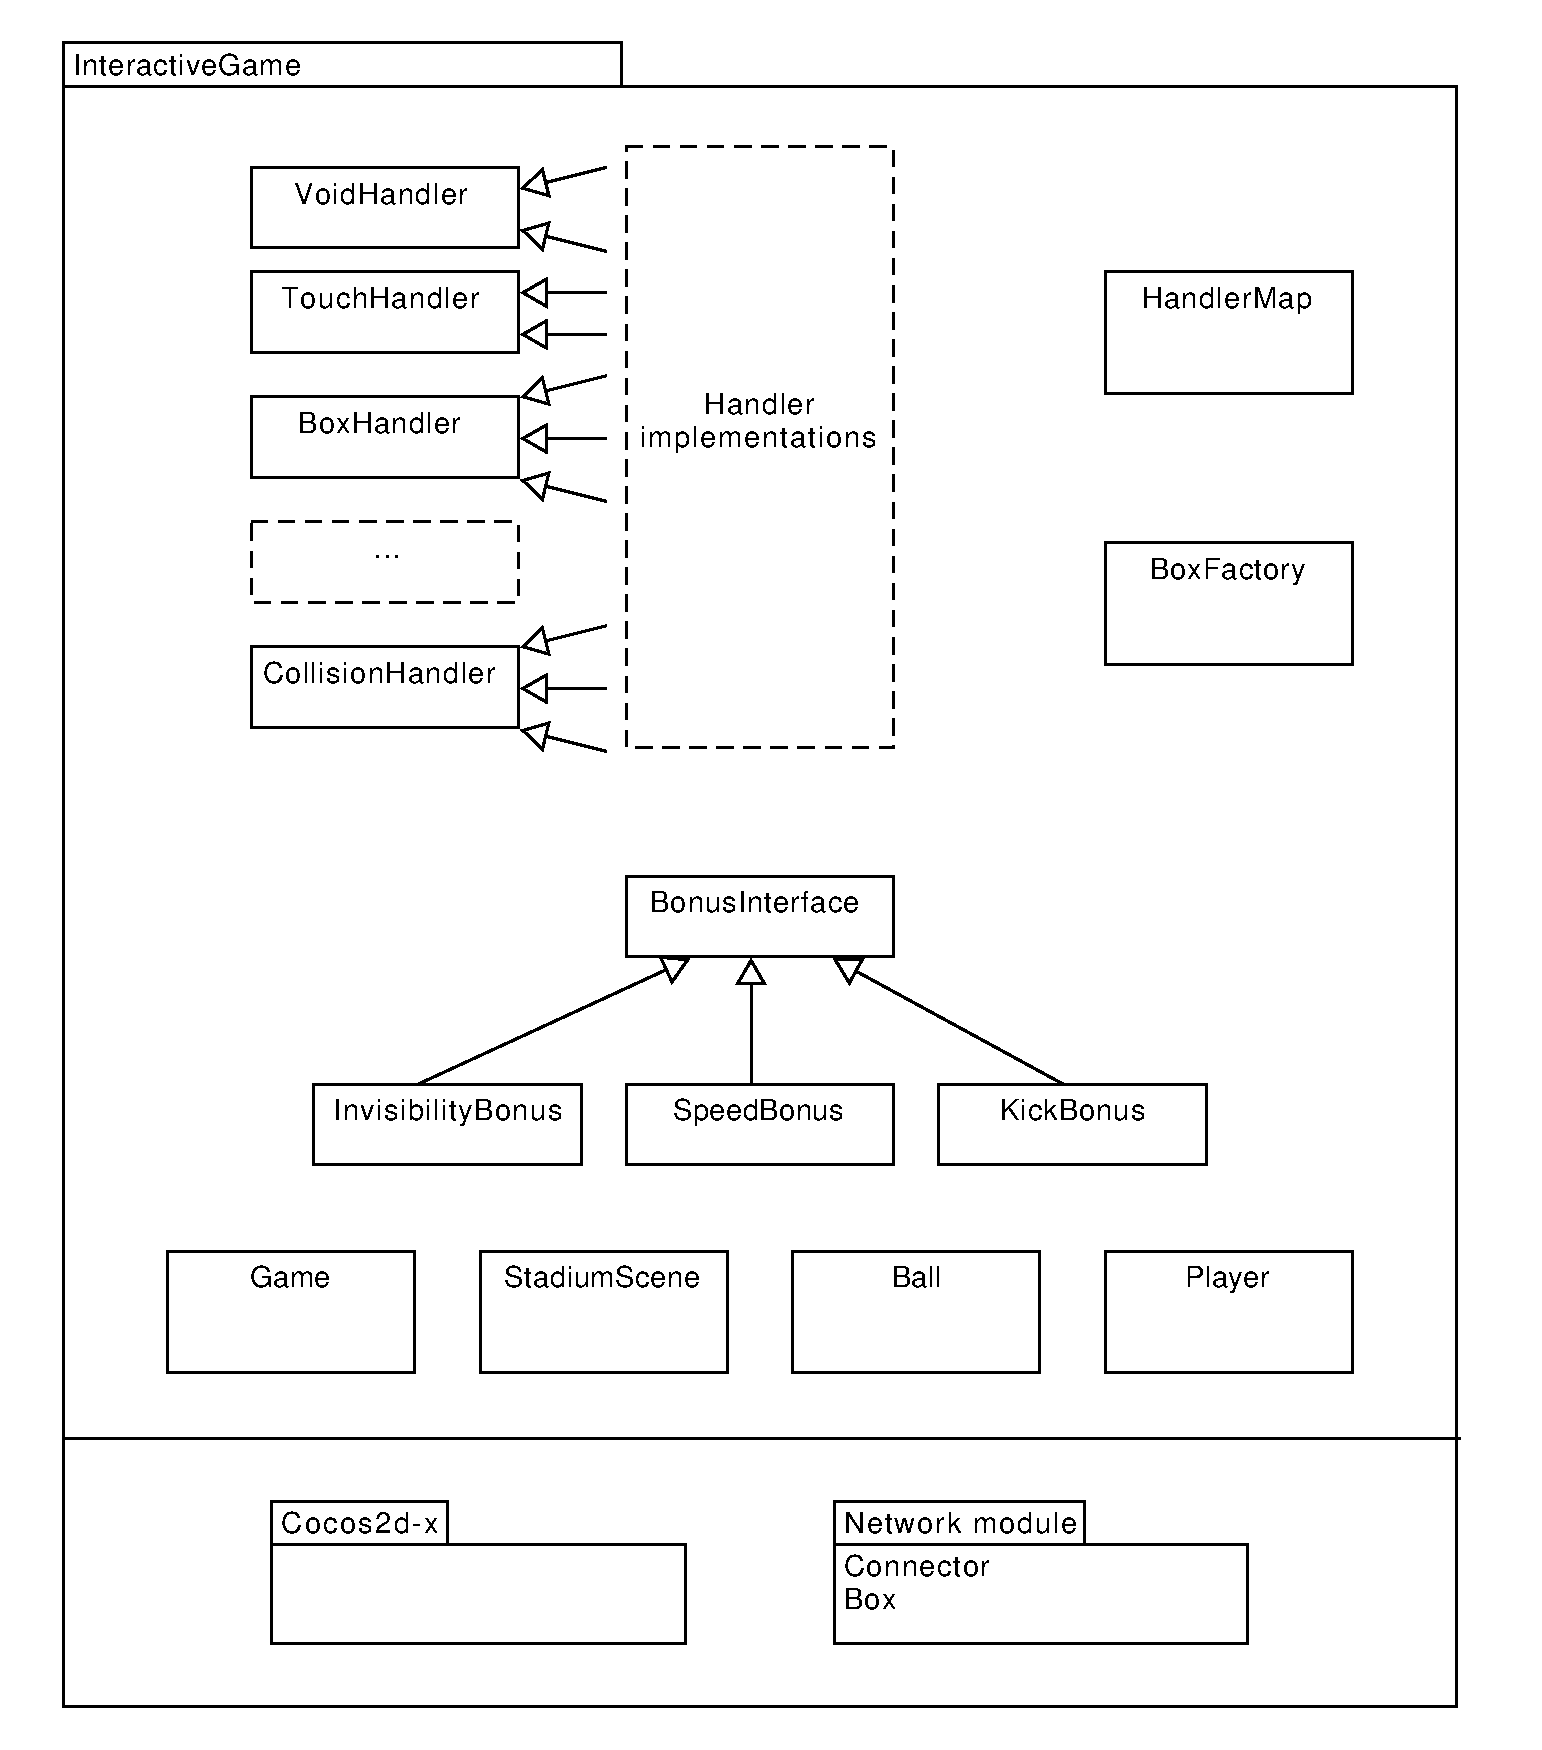
\includegraphics[width=\textwidth]{game_architecture}
\caption{Architektura hry}
\end{figure}

\subsubsection{Herní bonusy}

Prvkem, který obohacuje celkovou hratelnost, jsou bonusy. Umožňují dočasné zvýhodnění hráče během zápasu změnou jeho vlastností na hřišti. 

Obecnou definici herního bonusu obsahuje abstraktní třída \code{BonusInterface}. Mezi její základní metody patří \code{activate()} a~\code{deactivate()}. Bonusy dále obsahují informace o~době, jak dlouho budou aktivní, kdo vzal daný bonus a~jakou má bonus grafiku. Návrh počítá se třemi implementacemi bonusů: rychlost, síla kopu a~neviditelnost.

Bonus rychlosti zvyšuje hráči maximální rychlost, jakou se může pohybovat po hřišti. Může tak doběhnout míč lépe než protivník nebo se rychleji přiblížit k~brance.
Podobně jako rychlost zvyšuje bonus kopnutí sílu, která bude aplikována na míč. Pokud hráč s~tímto bonusem vystřelí, míč letí rychleji a~může doletět přes značnou část celého hřiště.
Nejinteraktivnějším bonusem je neviditelnost. Hráč po sebrání bonusu zmizí z~hlavní obrazovky a~celé hřiště se mu zobrazí na mobilní obrazovce a~kromě toho může procházet skrz ostatní hráče. Neviditelný hráč získává velkou taktickou výhodu, může volněji manipulovat s~míčem a~překvapit protivníka svou pozicí na hřišti.

\subsection{Architektura ovladače}

Základní struktura ovladače je velmi podobná hře, jelikož využívá velké množství stejných komponent: Návrhový vzor Handler je použit jak ve hře, tak i~v~ovladači, obě aplikace spolu sdílí abstraktní části kódu, jen implementace konkrétních handlerů jsou odlišné. Stejně tak je využíván síťový modul a~sdílené jsou i~grafické zdroje. Proto se zde budu věnovat především odlišným prvkům.

Na rozdíl od hry ovladač obsahuje více herních scén (obrazovek). Konkrétně se jedná o~hlavní menu, obrazovku s~výběrem týmu, ovládací obrazovka a~scéna s~vykresleným hřištěm. Přechody mezi jednotlivými obrazovkami a~událostmi, které vyvolají přechody, popisuje diagram \ref{picture:controller_scenes}.

\begin{figure}[h]
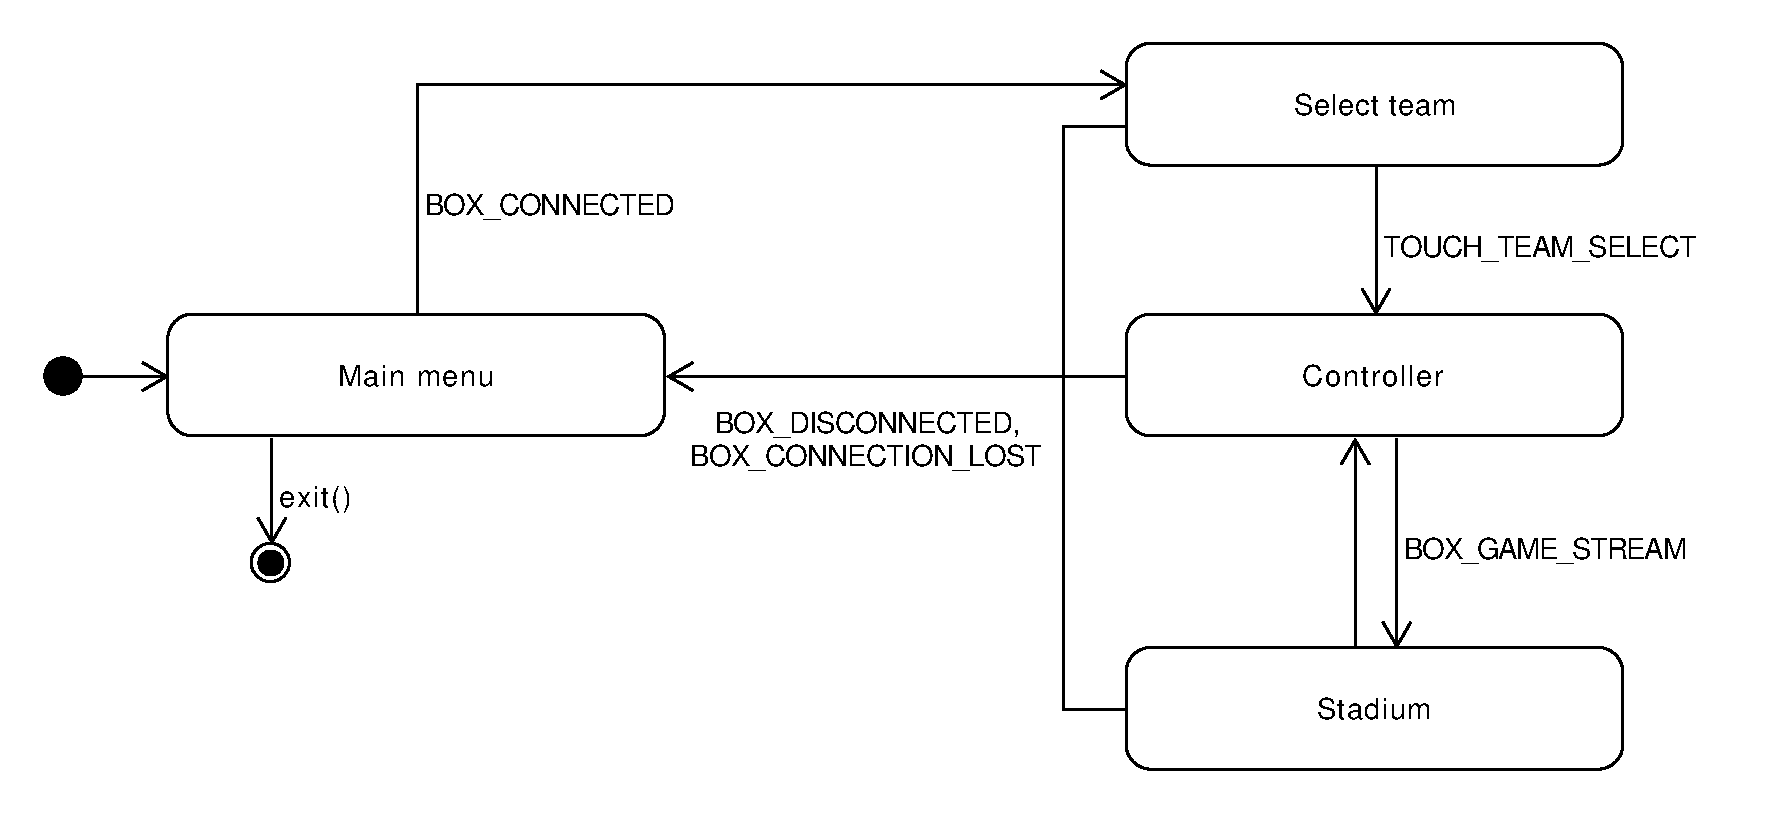
\includegraphics[width=\textwidth]{controller_scenes}
\caption{Události přechodů mezi obrazovkami}
\label{picture:controller_scenes}
\end{figure}


Hlavní menu je první zobrazenou scénou po spuštění ovladače. Obsahuje nastavení hráčovy přezdívky, aktivace vibrací a~seznam nalezených serverů. Po kliknutí na vybraný server naváže ovladač spojení s~hrou a~zobrazí volbu týmu. Hráč si může zvolit ze dvou týmů (červený nebo modrý), případně si nechat určit tým automaticky. Po přiřazení týmu se zobrazí ovládací obrazovka, které dominuje velké tlačítko pro kopnutí do míče. Pokud vezme hráč během zápasu bonus neviditelnosti, zobrazí se mu na mobilním displeji totožné hřiště jako na hlavní obrazovce. Kopnout do míče při neviditelnosti lze dotykem libovolně na obrazovce, aby se předešlo stínění prstem v~místě, kde zrovna probíhá hra. V~případě odpojení se ovladač vrátí do hlavního menu a~v~případě ztráty spojení zobrazí chybovou hlášku.

\subsection{Komunikace mezi ovladačem a~hrou}

Vzhledem k~použití handlerů v~systému je možné návrh síťové komunikace realizovat s~jejich využitím: přijetí síťové zprávy vyvolá herní událost a~následně proběhne její zpracování. Vzhledem k~tomu, že síťové zprávy i~události jsou rozlišeny identifikátorem, je možné tyto identifikátory konsolidovat a~použít pro událost i~zprávu totožný identifikátor. 

Nejběžnějším scénářem komunikace je sled následujících kroků: vyhledání her v~lokální síti, připojení na zvolenou hru, volba týmu, spuštění hry a~poté herní komunikace. V~případě aktivace bonusu neviditelnosti začne hra posílat informace o~svém stavu danému ovladači, aby byl schopen vykreslit kompletní hru na své obrazovce.

Stavový diagram \ref{picture:communication_states} přehledně zobrazuje jednotlivé stavy hry i~ovladače z~hlediska síťové komunikace a~zachycuje, kdy se posílají důležité informace.

\begin{figure}[h]
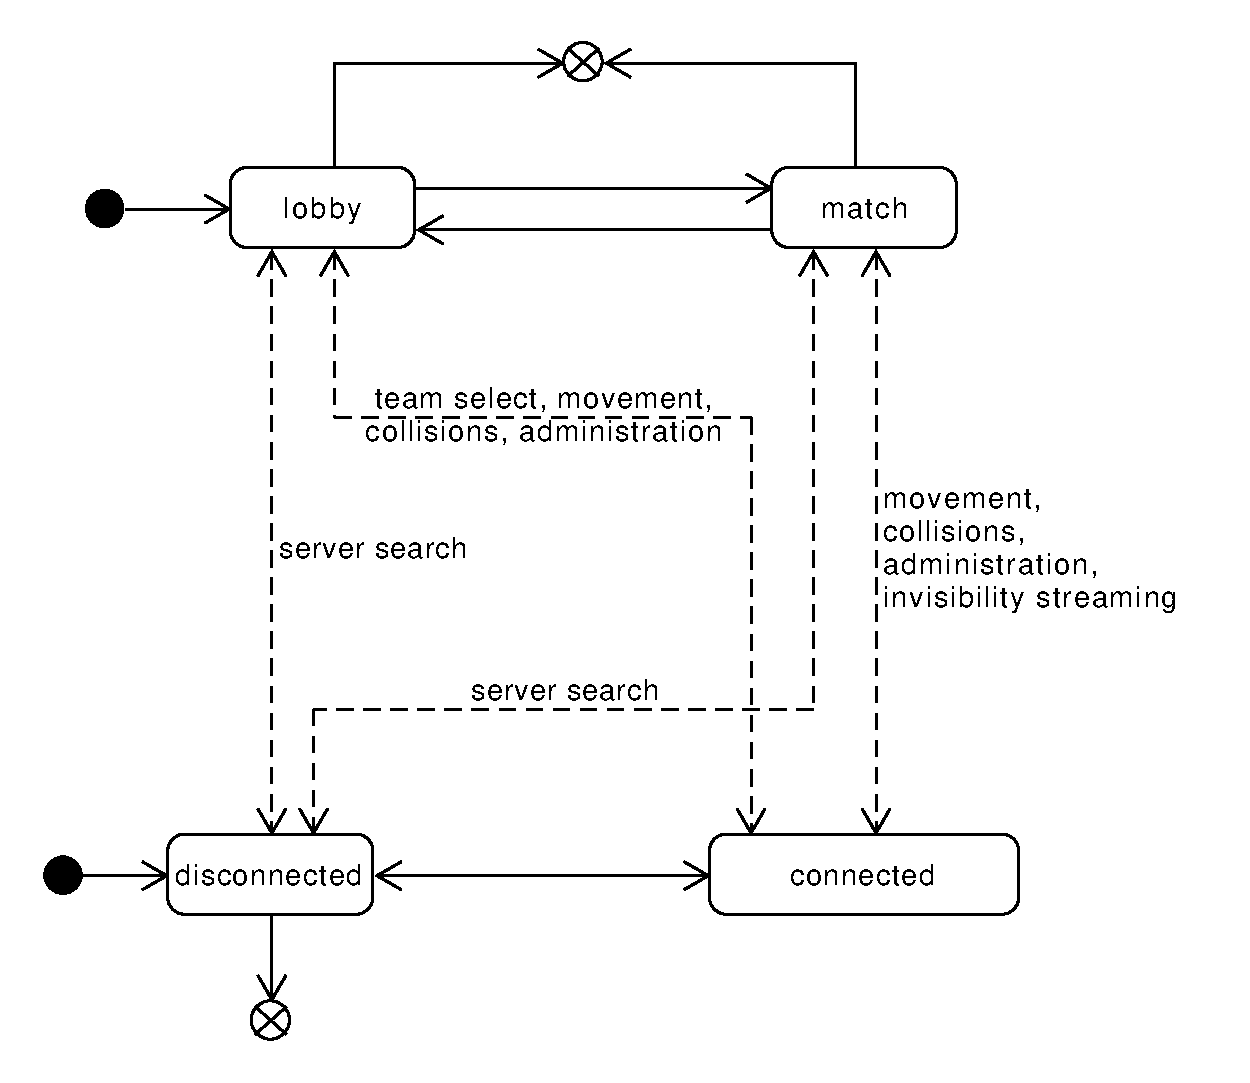
\includegraphics[width=\textwidth]{communication_states}
\caption{Komunikační stavy hry a~ovladače}
\label{picture:communication_states}
\end{figure}

Nedílnou součástí návrhu celého systému je zpracování dat ze zpráv. Některé zprávy žádná data neobsahují, informační hodnotu představuje pouze identifikátor Boxu. Jiné obsahují jednoduchý textový řetězec a~jejich zpracování je pak triviální, ale existují i~zprávy s~komplexní strukturou a~tím pádem i~složitým zpracováním. Takovou zprávou je například stav hry posílaný ze serveru pro vykreslování hry při neviditelnosti. Zpráva musí obsahovat informace o~všech viditelných hráčích (pozice, rychlost a~směr pohybu, barva týmu), míči a~některé další informace. Takováto zpráva musí mít definovanou pevnou strukturu. Protože se obsah může měnit (např. když se změní počet hráčů), její návrh vyžaduje hlubší analýzu.

Původním záměrem, jak zpracovávat zprávy, bylo vytvořit vlastní parsovací systém pro každou zprávu. Ukázalo se však, že tento způsob je nedostačující především u~složitějších zpráv. Jako lepší varianta se nabízelo využití existujících technologií pro serializaci dat. Z~několika vhodných řešení jsem si zvolil knihovnu \textit{Protocol Buffers} vyvíjenou společností Google. Jedná se o~multiplatformní knihovnu s~otevřeným zdrojovým kódem, která umožňuje definici struktury zprávy, její serializaci a~deserializaci a~použití více programovacími jazyky současně. \cite{protobuf} Použití Protocol Buffers je velmi jednoduché. Nejprve je třeba definovat strukturu zprávy s~určenou syntaxí a~poté v~příkazové řádce vygenerovat soubory s~požadovaným zdrojovým kódem (v~tomto případě C++). Tyto vygenerované soubory se poté importují do projektu a~je možné je přímo využívat.

Využití Google Protocol Buffers elegantně vyřešilo problém zpracování zpráv a~umožnilo velmi jednoduše specifikovat komplexní struktury dat posílané po síti.

V~definici zprávy lze určit, zda se proměnná ve zprávě musí vyskytovat (parametr \code{required}), nebo se nutně vyskytovat nemusí (\code{optional}), či může existovat několik instancí (\code{repeated}), ale také nemusí být žádná. Následující ukázka ilustruje definici jednoduché zprávy v~systému Protocol Buffers:

\begin{figure}[h]
\code{message Person \{ \\
\tab required string name = 1; \\
\tab required int32 id = 2; \\
\tab optional string email = 3; \\
\tab repeated string address = 4; \\
\}}
\end{figure}

Pokud je nutné změnit strukturu zprávy, stačí upravit soubor s~definicí a~znovu vygenerovat zdrojové soubory. Není potřeba ručně měnit algoritmus parsování zprávy, jako by tomu bylo při použití vlastního primitivního parsování.

\subsection{Shrnutí}

Ve fázi návrhu jsem vytvořil základní strukturu síťového modulu včetně zpracování zpráv, hry a~ovladače. Následující fází je implementace: naprogramování navržených funkcionalit a~vytvoření funkčního systému.

\section{Implementace}

Přesto, že implementace zabrala značnou část tvorby této práce, není možné obsáhnout všechny části tvorby hry a~ovladače, proto se zde budu zabývat především těmi částmi, které jsou něčím zajímavé, komplikované nebo důležité pro celý systém.

\subsection{Vývojové prostředí}

Celý vývoj probíhal v~operačním systému OS X, konkrétně ve vývojovém prostředí Xcode. Jednalo se o~mou první zkušenost s~tímto prostředím i~s~operačním systémem OS X, proto byla tvorba v~počátcích komplikovaná, později však vývoj probíhal bez problémů a~začal jsem dokonce využívat výhod, které mi toto prostředí nabízelo.

Kromě vývojového prostředí jsem hojně využíval příkazovou řádku, především pro kompilaci projektu pro operační systém Android.

\subsection{Struktura projektu, integrace knihoven}

Prvním krokem každé implementace je založení projektu. Podle návodů jsem vytvořil prázdný projekt s~herním engine Cocos2d-x. Do tohoto projektu jsem poté importoval knihovnu RakNet a~vytvořil modul pro síťovou komunikaci. Přesto, že vývoj tohoto modulu probíhal z~důvodu praktičnosti sloučeně se zbytkem hry, byl vyvíjen tak, aby jej bylo možné snadno importovat do libovolné jiné aplikace.

Vytvořil jsem tedy 2 projekty: jeden pro hru na PC a~druhý pro mobilní ovladač. Oba projekty odkazují na stejné zdrojové soubory síťového modulu a~změna v~něm se tak projeví v~obou aplikacích. Kromě toho sdílí projekty také několik dalších souborů, z~nichž nejvýznamnější je objekt \code{StadiumScene} obsahující implementaci fotbalového hřiště. Sdílení některých souborů ilustruje obrázek \ref{picture:source_sharing}.

\begin{figure}[h]
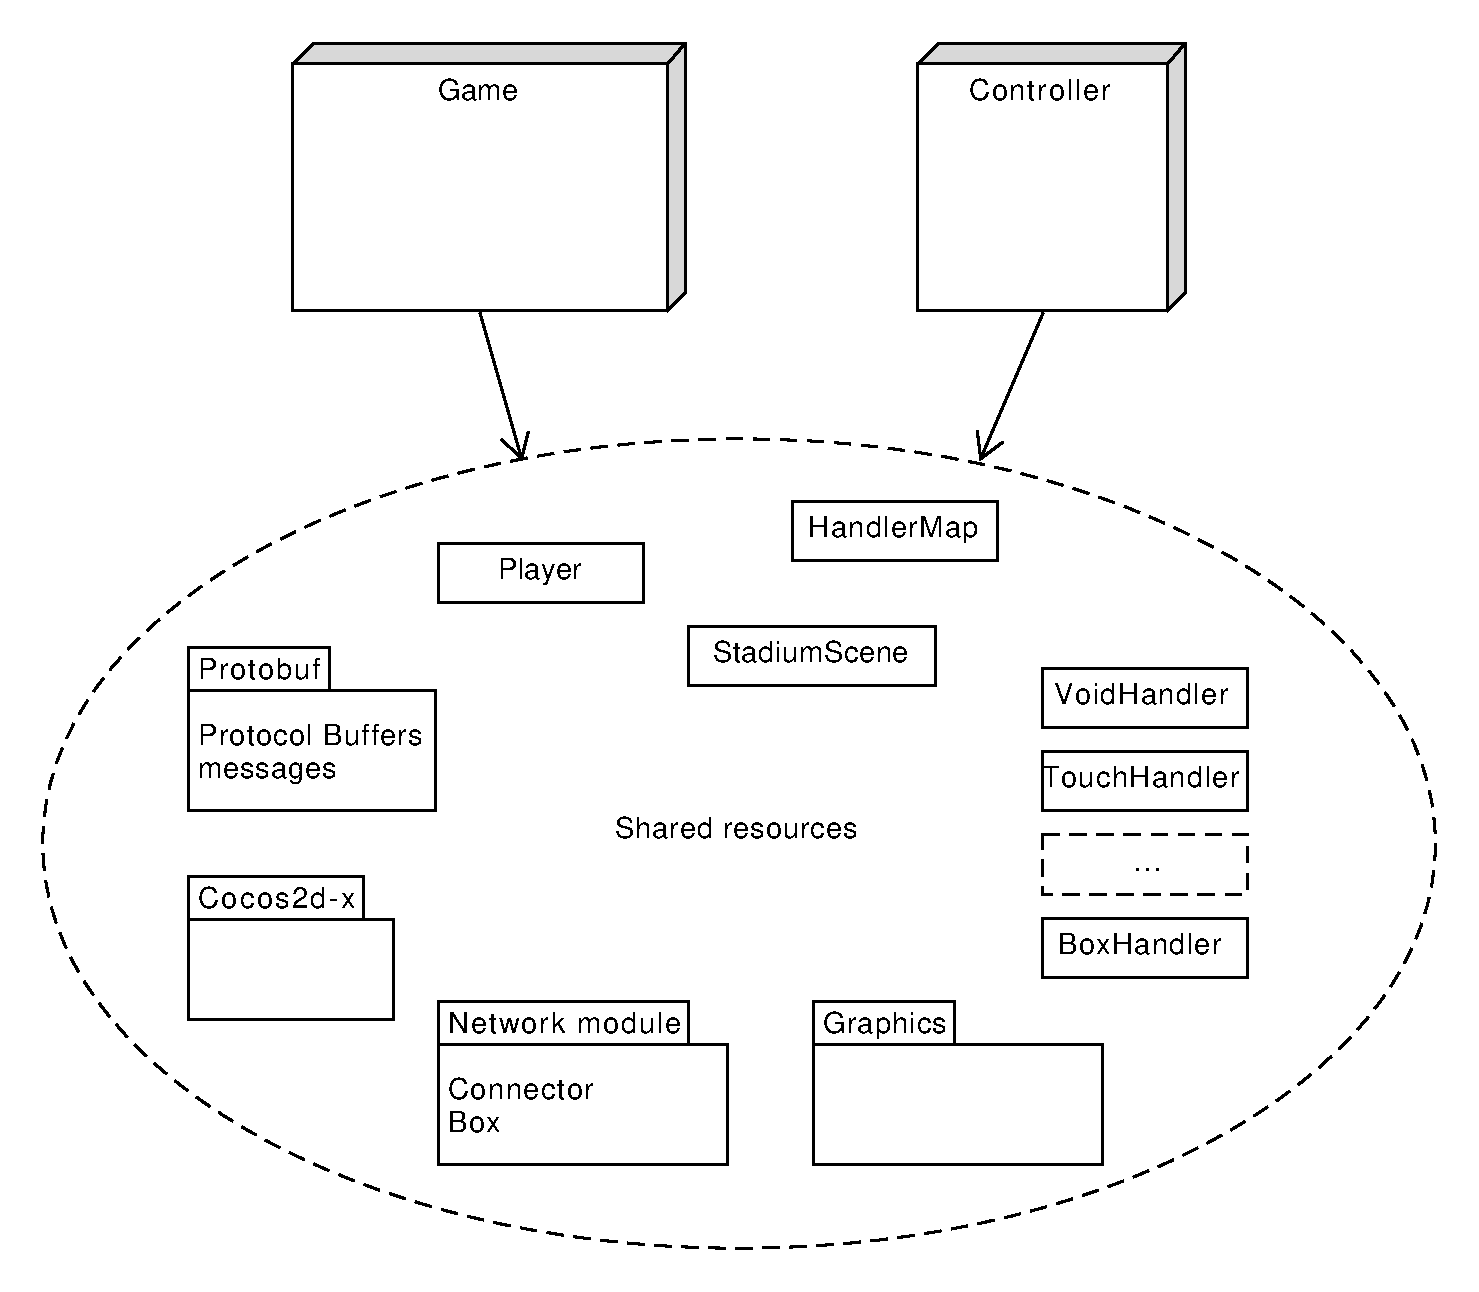
\includegraphics[width=\textwidth]{source_sharing}
\caption{Sdílení částí aplikace mezi hrou a~ovladačem}
\label{picture:source_sharing}
\end{figure}


\subsection{Síťový modul}

Implementace síťového modulu probíhala bez větších komplikací. Během studování knihovny RakNet jsem vytvořil testovací aplikace \textit{klient} a~\textit{server}, abych si vyzkoušel práci s~knihovnou. Velmi kvalitním zdrojem informací byla sada ukázkových programů nacházející se přímo v~distribuci knihovny. Programy jsou velmi dobře zdokumentované a~pomáhají pochopit daný kód.

\subsection{Připojení nového hráče}

Stěžejním krokem síťové komunikace je navázání spojení s~ovladačem. V~této sekci popíšu typický průběh navazování spojení z~pohledu systému:

\begin{enumerate}
	\item Hledání serverů: Ovladače periodicky posílají dotazovací zprávu na všesměrovou adresu v~lokální síti.
	\item Odpověď serverů: Herní servery, které přijaly dotazovací zprávu, odpovídají zprávou obsahující název serveru.
	\item Připojení na server: Ovladač zobrazuje nalezené servery a~po kliknutí na vybraný server s ním naváže aktivní spojení.
	\item Volba týmu: Ovladač je sice spojen se serverem, hráč se však stále nezobrazil na hřišti, musí si totiž nejprve zvolit tým. Provedená volba se odešle na server a~hráč je zobrazen na hřišti.
	\item Admin: Pokud je hráč první připojený, server mu odešle dodatečnou informaci, že má ovladač práva na správu hry.
	\item Spojení je navázáno, ovladač může volně komunikovat se hrou.
\end{enumerate}

Číslování jednotlivých kroků koresponduje pro lepší přehlednost s~kroky v~diagramu \ref{picture:connection}, který názorně ilustruje připojení nového hráče. 

\begin{figure}[h]
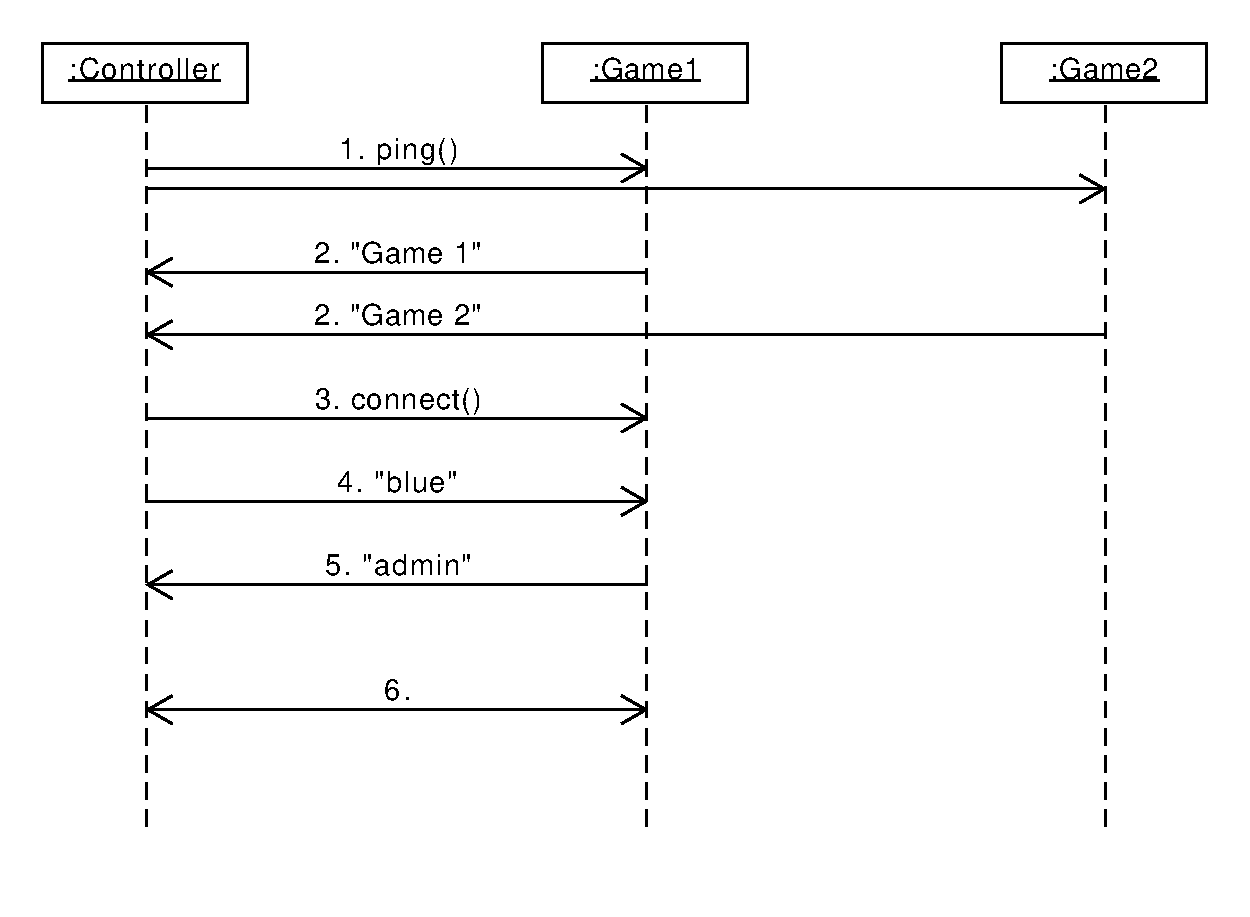
\includegraphics[width=\textwidth]{connection}
\caption{Připojení nového hráče}
\label{picture:connection}
\end{figure}

\subsection{Fyzikální engine}

Jednou z~funkcí knihovny Cocos2d-x je simulace chování objektů za pomoci integrovaného fyzikálního enginu. Herní princip fotbalu vychází ze simulace reálného světa, proto je zde fyzikální engine hojně využíván. Nejdůležitější prvky v~tomto případě tvoří objekty, jejich kolize a~detekce překryvu.

Fyzikální objekt obsahuje 2 elementy: tvar a~definice materiálu. Materiál má 3 složky: hustota, pružnost a~tření. Ve hře jsou fyzikálními objekty hráči, míč, branky, okraje hřiště a~detektory gólu. U~každého fyzikálního objektu lze definovat, s~jakým typem jiných fyzikálních objektů může kolidovat (například srážka dvou hráčů). Použití této definice je výhodné pro detekci gólu (obrázek \ref{picture:goal_detector}): do prostoru branky jsou umístěny neviditelné fyzikální objekty reprezentující detektory gólu, se kterými sice nekoliduje ani hráč, ani míč, ale je detekován překryv dvou objektů. Pokud se míč překryje s~detektory, vyvolá se událost gólu a~je přičten bod příslušnému týmu. Pohyb míče i~případného hráče v~brance je však neovlivněn.

\begin{figure}
\center
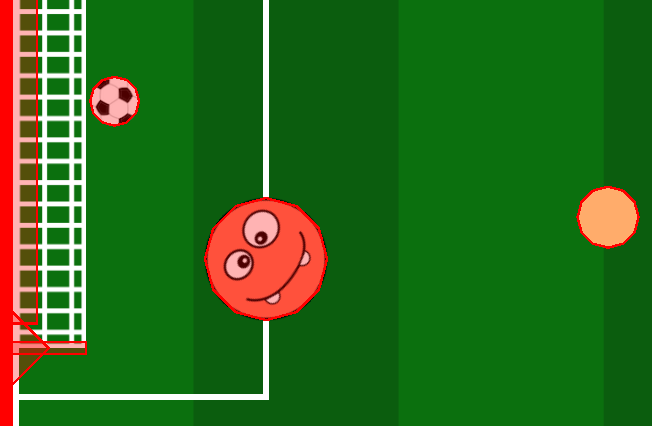
\includegraphics{goal_detector}
\caption{Zobrazení fyzikálních objektů a~detektoru gólu}
\label{picture:goal_detector}
\end{figure}

Dalším příkladem je bonus neviditelnosti: Pokud jej hráč vezme, změní se jeho definice kolizí a~přestane kolidovat s~ostatními hráči. Přesto, že je na hřišti neviditelný, jeho fyzikální reprezentace se pohybuje po hřišti a~kolize s~míčem tak funguje zcela normálně.

\subsection{Neviditelnost}

Stěžejní funkce, která výrazně obohacuje interaktivitu v~porovnání s~klasickými ovladači, je projekce kompletní herní scény na mobilní obrazovku při aktivním bonusu neviditelnosti. Její realizace s~sebou přinesla několik komplikací, které jsou podrobně rozebrány v~následující části. 

\subsubsection{Poměr stran hřiště}

Při snaze o~co nejvěrnější zobrazení stejného hřiště v~mobilním telefonu i~ve hře se logicky nabízí otázka, jak efektivně sdílet zdrojový kód mezi oběma platformami. Použití identického herního enginu tuto potřebu zjednodušuje, ale je potřeba vytvořit dostatečně obecné třídy a~umožnit jejich modifikaci pro potřeby dané platformy. Jako první byla vytvořena třída \code{StadiumScene} a~\code{Player} pouze na PC. Ukázalo se však, že přes veškeré výhody herního enginu existují komplikace, které zabraňují bezproblémovému použití stejného zdrojového kódu:

První komplikací bylo použití herních handlerů přímo ve \code{StadiumScene}. Mobilní platforma disponuje odlišnými implementaci handlerů, proto nebylo možné projekt zkompilovat. Oprava této chyby spočívala v~přesunu použití handleru do třídy \code{Game}. Třída \code{StadiumScene} se tak stala nezávislou na herních událostech a~bylo ji možné importovat do mobilní aplikace.

Druhý, avšak komplikovanější problém představovala rozdílnost herních obrazovek, zejména různorodost poměrů stran. Návrh hřiště počítá s~tím, že se hra bude snažit přizpůsobit rozměry hřiště monitoru tak, aby byla vyplněna celá plocha obrazovky. Například pokud hra běží na monitoru s~poměrem stran 16:9, herní hřiště bude mít totožný poměr stran. Komplikace nastávají, pokud se do hry připojí zařízení s~odlišným poměrem stran. Vzhledem k~tomu, že rozměry mobilních displejů jsou značně rozdílné, je velká pravděpodobnost výskytu tohoto problému. Hřiště v~mobilním displeji se, podobně jako u~PC, vykreslí přes celou obrazovku a~při rozdílných poměrech stran vznikají odchylky od skutečné polohy. To způsobuje nepřesnou hru či přesah objektu \uv{za hřiště}.

\begin{figure}
\center
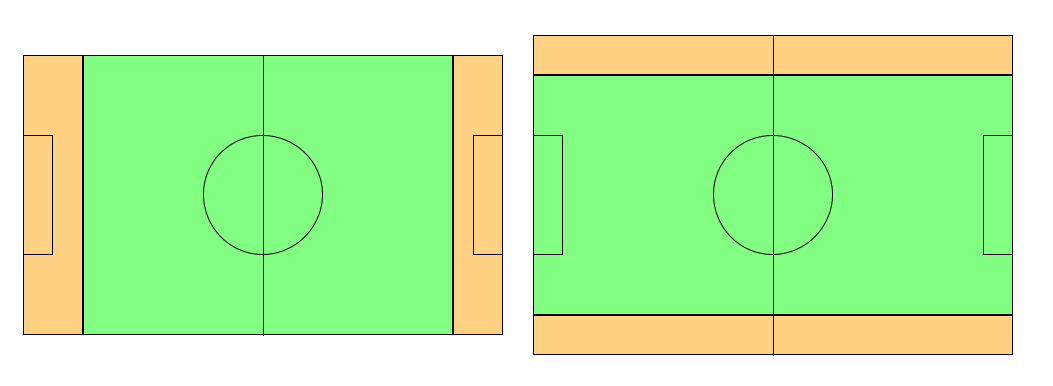
\includegraphics[width=\textwidth]{stadium_proportions_2}
\caption{Přesahy hřiště při různých poměrech stran}
\label{picture:stadium_proportions}
\end{figure}

Řešení tohoto problému spočívá ve dvou krocích. Prvním z~nich je odeslání rozměrů hřiště do mobilního telefonu. Hřiště se vykreslí s~totožnými rozměry jako na PC. To ale způsobuje přesah hřiště přes ty strany, které jsou na mobilním displeji menší než na PC. Přesahy ilustruje obrázek \ref{picture:stadium_proportions}, oranžová barva vyznačuje přesahující oblasti v~mobilním displeji. Pro zobrazení těchto oblastí jsem upravil vykreslování scény, aby se hřiště posouvalo v~závislosti na pozici hráče a~byly tak skryty jen nejvzdálenější části herní plochy. Tyto úpravy ale musely být vytvořeny nad samotnou třídou \code{StadiumScene}, aby neovlivnily vykreslování na PC.

\subsubsection{Vykreslování hráčů v~mobilní obrazovce}

Jako velmi zajímavou část během vývoje považuji ladění vykreslování hráčů na mobilním displeji. Aktivní bonus neviditelnosti periodicky posílá informace o~hře, jejíž součástí jsou také data o~jednotlivých hráčích. Na počátku vývoje obsahovaly tyto údaje pouze souřadnice hráče na hřišti. Tyto souřadnice pak používá ovladač pro nastavení pozice hráče na mobilním displeji. Při testování se však ukázalo, že tento návrh je téměř nepoužitelný: pohyb hráčů byl velmi trhaný, nepomohlo ani zvýšení frekvence posílání zpráv (z~30 na 60 zpráv za vteřinu) a~je proto potřeba vykreslování optimalizovat. Obrázek \ref{picture:player_rendering_1} znázorňuje pozice hráče přijaté po síti a~ilustruje nedostatečnost tohoto řešení. Jednotlivé pozice jsou nepravidelně vzdáleny. Překreslování tak netvoří dojem plynulosti.

\begin{figure}[h]
\center
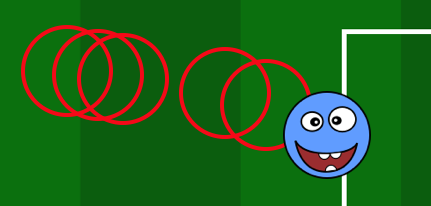
\includegraphics[width=\textwidth]{player_rendering_1}
\caption{Trhané vykreslování hráče}
\label{picture:player_rendering_1}
\end{figure}

Pro docílení plynulejšího pohybu jsem přidal do zprávy o~hráčích informaci o~vektoru pohybu. Z~dat se tak dala rekonstruovat nejen pozice, ale i~rychlost a~směr pohybu. Hráč na mobilní obrazovce se tedy pohyboval i~v~případě, že delší dobu nebyla přijata zpráva s~aktualizovanými údaji. Toto řešení vylepšilo celkový dojem z~vykreslování, stále se však objevoval trhaný pohyb a~občasné uskakování hráčů, byť v~menší míře.

\begin{figure}[h]
\center
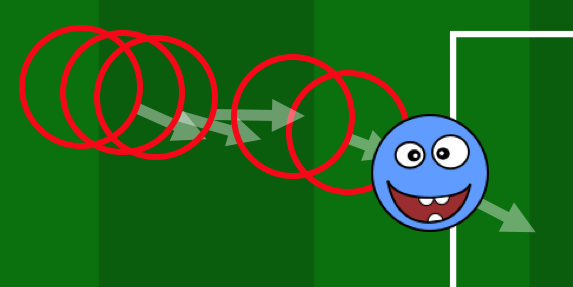
\includegraphics[width=\textwidth]{player_rendering_2}
\caption{Vykreslování hráče s~predikcí pohybu}
\label{picture:player_rendering_2}
\end{figure}

Protože bylo při tvorbě zprávy s~daty o~hráčích nastaveno odesílání a~přijímání zpráv bez zajištění spolehlivosti, kromě ztrát zpráv mohlo také docházet ke změně pořadí přijatých zpráv. Ztráta zpráv v~tomto případě nepředstavuje zásadní problém, jelikož neaktuální zprávy nejsou z~hlediska hry informačně hodnotné, komplikaci představuje změna pořadí. \uv{Starší} zprávy, které se dostanou před ty novější, mohou způsobit \uv{přeskakování} hráčů: Pokud přijdou dvě zprávy v opačném pořadí, hráč se nejprve přesune na starší místo (do protipohybu) a~poté zpět na správné místo. Tento problém vyřešilo jednoduché nastavení spolehlivosti zprávy na \code{UNRELIABLE\_SEQUENCED}, což způsobilo zahazování neaktuálních paketů a~elegantně vyřešilo problém s přeskakováním.

Zprávy o~hráčích nyní poskytují všechny informace potřebné pro vykreslení. Další vylepšování plynulosti se proto týkaly ovladače. Predikce pohybu s~využitím aktuální rychlosti vykazuje nedostatky ve chvíli, kdy hráč změní rychlost nebo směr pohybu a~zpráva s~touto informací přijde se zpožděním. Tato situace způsobuje zmiňované trhání. Způsobem, jak eliminovat toho trhání, je plynulá změna pozice pomocí animace objektu. Při zpracování nově přijaté zprávy se tak vypočítá vektor změny přijaté pozice od pozice na mobilním displeji. Z~toho se vytvoří animace, která přesune objekt hráče relativně o~vzdálenost vypočítaného vektoru. Zároveň však zůstane zachována predikce pohybu. 

\begin{figure}[h]
\center
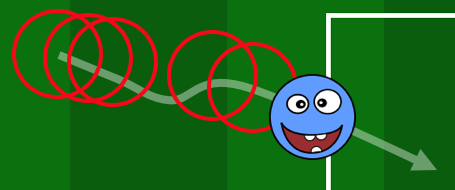
\includegraphics[width=\textwidth]{player_rendering_3}
\caption{Vykreslování s~predikcí pohybu a~plynulou korekcí}
\label{picture:player_rendering_3}
\end{figure}

Kombinace všech těchto vylepšení splňuje požadavky na plynulost pohybu, který je tak téměř identický jako na hlavní obrazovce. Výsledné řešení ilustruje obrázek \ref{picture:player_rendering_3}.

\subsection{Shrnutí}

Ve fázi implementace byl podle návrhu vytvořen funkční systém. Obě aplikace se podařilo vytvořit podle očekávání, stěžejní části a~případné komplikace zde byly rozebrány do větších podrobností. 

\section{Testování}
\label{section:testing}

Následující sekce se věnuje testování software a~to jak automatické, tak manuální. Je sice zařazena až po fázi implementace, některé testy však probíhaly souběžně s~implementací. 

\subsection{Unit testy}

Základní formou testování jsou automatizované testy, tzv. \textit{unit testy}. Pomocí nich se kontroluje elementární fukčnost jednotlivých komponent a~funkcí. Pro implementaci jsem použil testovací framework \textit{Catch} \cite{catch}. Mezi jeho výhody patří velmi snadná integrace a~velké množství testovacích maker. Následující ukázka zobrazuje jeden z~automatických testů síťového modulu, který kontroluje správnou inicializaci třídy \code{Box}:

\begin{verbatim}
TEST_CASE("GameNet tests")
{
    SECTION("Box") 
    { 
        GameNet::Box * box = nullptr;
        
        // string to box
        box = GameNet::Box::create("test");
        REQUIRE( box->getData().compare("test") == 0 );
        box->deallocate();
        
        // packet to box
        RakNet::Packet * packet = new RakNet::Packet();
        packet->data = new unsigned char[5];
        packet->length = 5;
        memcpy(packet->data, "\0test", 5*sizeof(char));
        box = GameNet::Box::create(packet);
        REQUIRE( box->getData().compare("test") == 0 );
		
        // custom dealloc - not the "real" RakNet packet
        delete [] box->getPacketData();
        delete [] packet->data;
        delete box;
    }
}
\end{verbatim}

Vzhledem k~vývoji v~prostředí Xcode jsou automatické testy implementovány na platformách iOS a~Mac OS X. Toto řešení splňuje požadavky uvedené v~návrhu hry, je zahrnuta alespoň jedna mobilní a~jedna počítačová platforma. Rozšíření testování i~na Android je komplikovanější a~přesahuje požadavky této práce.

Při vývoji pro více mobilních platforem by však bylo vhodné automaticky testovat všechny platformy, aby se zamezilo chybám způsobeným např. odlišnou architekturou či hardware.

\subsection{Testy paměti}

Dalším systémovým testem je kontrola správné alokace paměti. Vzhledem k~tomu, že celý systém je napsán v~jazyce C++, nejsou paměťové chyby automaticky kontrolovány. Herní engine Cocos2d-x sice pracuje s~pamětí efektivně, přesto však během vývoje docházelo v~aplikacích ke špatné dealokaci. Za následek této chyby bylo nekontrolovatelný růst spotřeby operační paměti.

Velké zásluhy na vyřešení těchto problémů mají integrované nástroje ve vývojovém prostředí Xcode. Ty umožňují kontrolovat správu paměti za běhu programu a~zobrazují špatně uvolněnou paměť v~reálném čase dokonce i~s~detekcí, na jakém místě v~kódu k~úniku došlo. Tímto způsobem bylo možné efektivně odstranit příčiny chyb a~zajistit optimální správu paměti.

\subsection{Testování hratelnosti}

Důležitou fázi při vývoji počítačových her představuje testování hratelnosti. Jeho cílem je nastavení parametrů hry pro vyvážení obtížnosti, ovládání a~dalších metrik. Testování hratelnosti se účastnilo 12 lidí a~jejich poznatky byly konzultovány během hry či po ní.

\begin{figure}[h]
\center
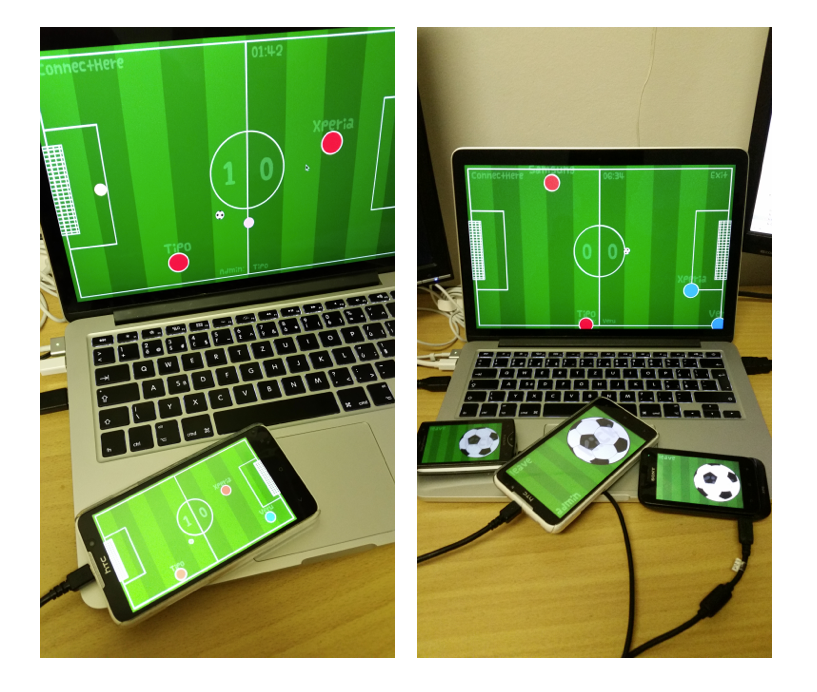
\includegraphics[width=\textwidth]{testing}
\caption{Testování hratelnosti}
\label{picture:testing}
\end{figure}

\subsubsection{Pohyb hráče}

V~případě fotbalu bylo nutné najít optimální model pohybu hráčů, aby hra nepůsobila jako pomalá nebo naopak příliš dynamická. V~počátcích návrhu měli hráči nízkou rychlost a~hra s~nižším počtem hráčů byla příliš zdlouhavá. Problém vyřešilo mírné zvýšení maximální rychlosti hráčů.

Jako druhý poznatek při ovládání hráči reportovali nepohodlné ovládání hry v~případě aktivního bonusu neviditelnosti. Aby viděli na displej, měli tendence naklánět telefon méně než při sledování hlavní obrazovky a~dosahovali tak nižších rychlostí. Toto bylo vyřešeno úpravou zpracování dat z~akcelerometru: pro dosažení maximální rychlosti stačí naklonit telefon méně než doposud. Hráči tak mohou sledovat obrazovku z~lepšího úhlu.

\subsubsection{Okraje hřiště}

Další problém během hraní se vyskytl v~situacích, kdy se míč dostal do okrajových částí hřiště: hrany a~rohy hřiště, případně vnější strana branek. Pokud míč následoval jeden nebo více hráčů, nebylo snadné míč dostat z~rohů zpět do hry. Tento problém negativně ovlivňoval herní zážitek.

Cílem vyřešení toho problému bylo předejít či eliminovat zaseknutí míče v~rozích a~jeho snadné odsunutí z~okraje hřiště. Pro tyto účely jsem využil možností fyzikálního enginu a~hřiště rozšířil o~další neviditelné objekty:

\begin{itemize}
	\item Zdvojení okrajů hřiště: první okraj je určen pro míč a~druhý (mírně přesahující \uv{za hřiště}) pro hráče. Ti se tak mohou dostat mírně za okrajovou čáru, což umožnilo lepší manipulaci s~míčem.
	\item Rohy hřiště: zabránit zaseknutí míče v~rozích se podařilo přidáním neviditelných objektů do rohů, které kolidují pouze s~míčem.
	\item Branky: podobně jako v~rozích jsem přidal neviditelné objekty ke hranám branek.
\end{itemize}

\begin{figure}[h]
\center
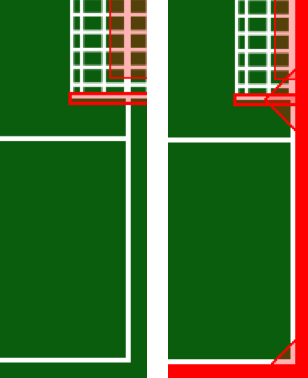
\includegraphics[width=\textwidth/2]{corners}
\caption{Oprava okrajů hřiště}
\label{picture:corners}
\end{figure}

Opravu tohoto problému ilustruje obrázek \ref{picture:corners}. Řešení elegantně eliminovalo problémy s~míčem a~vylepšilo celkovou hratelnost.

\section{Dokumentace}

Nedílnou součást každého softwarového produktu tvoří dokumentace. Jedná se o~soubor textů a~dalších materiálů, které provázejí celý vývoj projektu. V~této práci tvoří nejdůležitější části dokumentace požadavků, informační diagramy jednotlivých komponent a~dokumentace zdrojového kódu. Kromě toho je součástí také návod na kompilaci a~spuštění aplikací.

Dokumentace požadavků je uvedena v~kapitole \ref{section:requirements}. Obsahuje popis základních funkcionalit potřebných pro vytvoření funkčního systému.

Dokumentace zdrojového kódu zlepšuje přehlednost a~srozumitelnost kódu především pro vývojáře. V~definici metod a~rozhraní vysvětluje účel jejich použití a~v~implementaci pomáhá např. s~pochopením algoritmů či složitějších oblastí kódu. 

Kromě textového popisu je důležité také znázornění vztahů mezi komponentami a~jejich spolupráce. Vhodně navržený diagram může pomoci pochopit problematiku lépe než velké množství textu. Množství diagramů v~předešlých částech práce tak tvoří součást projektové dokumentace.

\section{Možnosti rozšíření}

Jako v~mnoha softwarových projektech zde existuje prostor pro další vývoj. Některé prvky nebyly implementovány, ať už z~důvodu časové náročnosti, nebo protože nespadají do nutných požadavků práce.

Jedním z~návrhů na vylepšení je grafika. Lepší zpracování obrázků, vytvoření více animací a~použití částicových efektů by hru vizuálně oživilo a~pomohlo tak k~intenzivnějšímu hernímu zážitku.

Dalším možností rozšíření je použití zvukových efektů. Ty nebyly z~časových důvodů implementovány, jejich nasazení umocní celkovou atmosféru hry.

Podobných návrhů na další vývoj existuje celá řada, například: nové typy herních bonusů, integrace herního serveru do mobilní obrazovky (server by tak mohl být použit v~mobilním zařízení například při připojení do externí obrazovky), vytvoření hráčů s~umělou inteligencí (využitelné, když je připojen lichý počet hráčů) a~mnoho dalších.

\section{Využití v dalších hrách}

Kromě rozšíření stávající hry umožňuje systém snadno vytvořit odlišnou hru. Nejzásadnějšímí kroky je vytvoření herních tříd, vlastní množiny událostí a~zpráv a~poté tvorba příslušných handlerů využívající tyto třídy a~zprávy.

\begin{conclusion}
	
V této bakalářské práci jsem se zabýval zkoumáním možností, jak ovládat PC hru pomocí chytrého telefonu. V~první kapitole jsem popsal nejběžnější herní ovladače a~jejich schopnosti a~porovnal je se senzory chytrých telefonů v~druhé kapitole. Součástí teoretické části bylo také nalezení podobných existujících řešení a~diskuse jejich vlastností.

Všechny tyto kapitoly sloužily jako teoretický základ pro analýzu a~realizaci softwarového projektu. Ten měl za cíl vytvořit systém pro interaktivní ovládání PC hry a~demonstrovat jeho schopnosti v~jednoduché hře. Tohoto cíle se podařilo dosáhnout vytvořením hry s~tematikou fotbalu. Softwarový projekt byl rozdělen na standardní fáze: analýza, návrh, implementace a~testování.

Systém vytvořený v~této práci pro podporu interaktivních her ulehčuje případný návrh dalších her. Není omezen na konkrétní herní žánr, jeho modularita jej předurčuje k~použití v~libovolném typu interaktivní hry. 

V~rámci bakalářské práce jsem využil poznatky získané při studiu, především z~oblastí softwarového projektu, objektového modelování a~síťové komunikace. Kromě toho považuji za osobní přínos první větší zkušenost s~herním enginem a~vývojem her. Z~dlouhodobého hlediska bych chtěl využít získané zkušenosti pro další výzkum způsobů ovládání her a~jejich interakce s~cílem propojit herní svět s~realitou. 
	
\end{conclusion}

\bibliographystyle{csn690}
\bibliography{mybibliographyfile}

\appendix

%\chapter{Seznam použitých zkratek}
%\printglossaries
%\begin{description}
%\end{description}

\chapter{Obsah přiloženého CD}

\begin{figure}
	\dirtree{%
		.1 readme.txt\DTcomment{stručný popis obsahu CD}.
		.1 bin\DTcomment{adresář se spustitelnou formou implementace}.
		.1 src.
		.2 impl\DTcomment{zdrojové kódy implementace}.
		.2 thesis\DTcomment{zdrojová forma práce ve formátu \LaTeX{}}.
		.1 text\DTcomment{text práce}.
		.2 thesis.pdf\DTcomment{text práce ve formátu PDF}.
%		.2 thesis.ps\DTcomment{text práce ve formátu PS}.
	}
\end{figure}

\end{document}
